% =====================================================================
%  Phase 2 paper  --  Team 6
%  Build:  cd phase2 && pdflatex phase2_paper && pdflatex phase2_paper
%  Every number in this file is produced by scripts/compute_results.py
%  (costs, bytes) or scripts/crt_revocation_attack.py (attack check).
% =====================================================================
\documentclass[11pt,a4paper]{article}

\usepackage[T1]{fontenc}
\usepackage[utf8]{inputenc}
\usepackage{lmodern}
\usepackage{microtype}
\usepackage[a4paper,margin=2.2cm,headheight=14pt]{geometry}
\usepackage{amsmath,amssymb,amsthm}
\usepackage{xcolor}
\usepackage{graphicx}
\usepackage{booktabs,array,tabularx,multirow}
\usepackage{enumitem}
\usepackage{float}
\usepackage{caption}
\usepackage{titlesec}
\usepackage{fancyhdr}
\usepackage{pifont}
\usepackage{tcolorbox}
\tcbuselibrary{skins,breakable}
\usepackage{tikz}
\usetikzlibrary{arrows.meta,positioning,shapes.geometric,shapes.misc,fit,backgrounds,calc,shadows,decorations.pathreplacing}
\usepackage{pgfplots}
\usepackage{pgfplotstable}
\pgfplotsset{compat=1.17}
\usepackage[colorlinks=true,linkcolor=deep,citecolor=uavc,urlcolor=uavc]{hyperref}

% ---------------- palette ----------------
\definecolor{deep}{HTML}{0B3954}     % night sky  -- titles, TA
\definecolor{uavc}{HTML}{087E8B}     % teal       -- UAV tier (C1)
\definecolor{vehc}{HTML}{6A4C93}     % violet     -- vehicle tier (C2)
\definecolor{hoc}{HTML}{E07A1F}      % amber      -- handover tier (C3)
\definecolor{bad}{HTML}{C81D25}      % red        -- flaws, attacks
\definecolor{good}{HTML}{2A9D3F}     % green      -- fixed / holds
\definecolor{soft}{HTML}{F2F6F8}     % light panel
\definecolor{ink}{HTML}{1F2933}

\color{ink}
\captionsetup{font=small,labelfont={bf,color=deep}}
\setlist{itemsep=2pt,topsep=4pt}

% ---------------- headings ----------------
\titleformat{\section}{\Large\bfseries\sffamily\color{deep}}{\thesection}{0.8em}{}
\titleformat{\subsection}{\large\bfseries\sffamily\color{uavc}}{\thesubsection}{0.7em}{}
\titleformat{\subsubsection}{\normalsize\bfseries\sffamily\color{ink}}{\thesubsubsection}{0.6em}{}
\pagestyle{fancy}\fancyhf{}
\fancyhead[L]{\small\sffamily\color{deep}Cutting the Cord -- Phase 2}
\fancyhead[R]{\small\sffamily\color{deep}Team 6}
\fancyfoot[C]{\small\sffamily\thepage}
\renewcommand{\headrulewidth}{0.4pt}

% ---------------- boxes ----------------
\newtcolorbox{whatbox}[1][]{enhanced,breakable,colback=uavc!6,colframe=uavc,boxrule=0.6pt,arc=2mm,
  fonttitle=\sffamily\bfseries,title={What this step does},#1}
\newtcolorbox{whybox}[1][]{enhanced,breakable,colback=hoc!7,colframe=hoc,boxrule=0.6pt,arc=2mm,
  fonttitle=\sffamily\bfseries,title={Why it is designed this way},#1}
\newtcolorbox{flawbox}[1][]{enhanced,breakable,colback=bad!5,colframe=bad,boxrule=0.6pt,arc=2mm,
  fonttitle=\sffamily\bfseries,#1}
\newtcolorbox{keybox}[1][]{enhanced,breakable,colback=deep!5,colframe=deep,boxrule=0.6pt,arc=2mm,
  fonttitle=\sffamily\bfseries,title={Key idea},#1}
\newtcolorbox{limitbox}[1][]{enhanced,breakable,colback=black!3,colframe=black!55,boxrule=0.6pt,arc=2mm,
  fonttitle=\sffamily\bfseries,title={Honest limitation},#1}
\newtcolorbox{stepbox}[2]{enhanced,breakable,colback=white,colframe=#1,boxrule=0.8pt,arc=2mm,
  fonttitle=\sffamily\bfseries,coltitle=white,colbacktitle=#1,title={#2}}

% ---------------- theorem-like ----------------
\theoremstyle{plain}
\newtheorem{theorem}{Theorem}
\newtheorem{lemma}{Lemma}
\newtheorem{proposition}{Proposition}
\theoremstyle{definition}
\newtheorem{definition}{Definition}
\newtheorem{finding}{Finding}

% ---------------- notation macros ----------------
\newcommand{\TA}{\mathsf{TA}}
\newcommand{\Ta}{\mathcal{T}_a}
\newcommand{\Tb}{\mathcal{T}_b}
\newcommand{\U}{\mathcal{U}}
\newcommand{\V}{\mathcal{V}}
\newcommand{\Ent}{\mathcal{E}}
\newcommand{\M}{\mathcal{M}}
\newcommand{\G}{\mathbb{G}}
\newcommand{\Zq}{\mathbb{Z}_q^{*}}
\newcommand{\Ppub}{P_{\mathrm{pub}}}
\newcommand{\Tpub}{T_{\mathrm{pub}}}
\newcommand{\PID}{\mathit{PID}}
\newcommand{\RID}{\mathit{RID}}
\newcommand{\ID}{\mathit{ID}}
\newcommand{\pk}{\mathit{pk}}
\newcommand{\sk}{\mathit{sk}}
\newcommand{\ep}{\mathit{ep}}
\newcommand{\ts}{\mathit{ts}}
\newcommand{\GK}{\mathit{GK}}
\newcommand{\VK}{\mathit{VK}}
\newcommand{\Tk}{\mathit{Tk}}
\newcommand{\hk}{\mathit{hk}}
\newcommand{\Enc}{\mathsf{Enc}}
\newcommand{\Dec}{\mathsf{Dec}}
\newcommand{\KDF}{\mathsf{KDF}}
\newcommand{\MAC}{\mathsf{MAC}}
\newcommand{\Hz}{H_0}
\newcommand{\Ho}{H_1}
\newcommand{\Ht}{H_2}
\newcommand{\Hd}{H_3}
\newcommand{\cat}{\,\|\,}
\newcommand{\yes}{\textcolor{good}{\ding{51}}}
\newcommand{\no}{\textcolor{bad}{\ding{55}}}
\newcommand{\halfmark}{\textcolor{hoc}{\ding{108}}}
\newcommand{\steplabel}[2]{\textcolor{#1}{\textsf{\textbf{#2}}}}

% ---------------- TikZ styles ----------------
\tikzset{
  ent/.style={draw=#1,fill=#1!12,very thick,rounded corners=3pt,minimum width=2.3cm,minimum height=0.9cm,
              align=center,font=\sffamily\small\bfseries,drop shadow={opacity=0.15}},
  ent/.default=deep,
  msg/.style={-{Stealth[length=2.6mm]},thick,draw=#1},
  msg/.default=ink,
  lbl/.style={font=\scriptsize\sffamily,fill=white,inner sep=1.5pt,align=center},
  life/.style={draw=black!30,dashed},
  act/.style={draw=#1,fill=#1!8,rounded corners=2pt,font=\scriptsize\sffamily,align=left,inner sep=3pt},
  tier/.style={draw=#1,fill=#1!5,rounded corners=6pt,dashed,thick},
}
\pgfplotsset{every axis/.append style={font=\small\sffamily,grid=major,grid style={black!10},
  legend style={font=\scriptsize\sffamily,draw=black!20,fill=white,fill opacity=0.9,text opacity=1},
  tick label style={font=\scriptsize\sffamily}, label style={font=\small\sffamily}}}

\pgfplotstableread[col sep=comma]{data/ga_cost.csv}\gacost
\pgfplotstableread[col sep=comma]{data/e2e.csv}\etoe
\pgfplotstableread[col sep=comma]{data/keybytes.csv}\keybytes
\pgfplotstableread[col sep=comma]{data/isolation.csv}\isolation
\pgfplotstableread[col sep=comma]{data/rekey.csv}\rekey

% =====================================================================
\begin{document}

% ---------------- title page ----------------
\begin{titlepage}
\begin{tikzpicture}[remember picture,overlay]
  \fill[deep] (current page.north west) rectangle ([yshift=-9.2cm]current page.north east);
  \foreach \x/\y/\c in {2.2/-2.2/uavc,4.0/-1.3/uavc,6.0/-2.6/uavc,15.5/-1.6/hoc,17.4/-2.8/vehc,13.6/-2.9/uavc}{
     \node[circle,fill=\c,minimum size=4pt,inner sep=0] at ([xshift=\x cm,yshift=\y cm]current page.north west) {};}
  \draw[white!40,thin,dashed] ([xshift=2.2cm,yshift=-2.2cm]current page.north west)--([xshift=4cm,yshift=-1.3cm]current page.north west)
       --([xshift=6cm,yshift=-2.6cm]current page.north west);
  \draw[white!40,thin,dashed] ([xshift=13.6cm,yshift=-2.9cm]current page.north west)--([xshift=15.5cm,yshift=-1.6cm]current page.north west)
       --([xshift=17.4cm,yshift=-2.8cm]current page.north west);
  \node[anchor=north west,text width=16.5cm,align=left,white] at ([xshift=2.2cm,yshift=-3.3cm]current page.north west)
   {{\sffamily\small PHASE 2 \;\textbullet\; RESEARCH GAP, PROPOSED FRAMEWORK AND ANALYSIS}\\[6pt]
    {\sffamily\bfseries\fontsize{30}{34}\selectfont Cutting the Cord}\\[6pt]
    {\sffamily\Large A Three-Tier, Authority-Independent Authentication and Key Management Framework for TUAV-Assisted Infrastructure-Less IoV}};
\end{tikzpicture}
\vspace*{8.6cm}

{\sffamily\large\textbf{Swaraj Kumar} (2025202016) \quad \textbf{Hritik Ranjan} (2025202031) \quad \textbf{Harsh Raj} (2025202005)}\\[3pt]
{\sffamily Team 6 \;\textbullet\; October 2026}

\vspace{0.6cm}
\begin{tcolorbox}[enhanced,colback=soft,colframe=deep,boxrule=0.5pt,arc=2mm,title={\sffamily\bfseries Abstract},fonttitle=\sffamily\bfseries]
\small
Tan, Zheng and Vijayakumar (IEEE T-ITS, 2023) propose a tethered UAV (TUAV) that replaces destroyed roadside units so that an
Internet of Vehicles (IoV) keeps working after a disaster. We studied the scheme equation by equation and found that it does not
achieve the property it is named for. Every authentication is relayed over a satellite link to a cloud Trusted Authority (TA), which
performs all the pairings, so authentication stops completely when that link is lost. Because the UAV credential depends only on
values the TA already knows, the TA can impersonate any UAV, which falsifies the claimed key-escrow resilience and non-repudiation.
We also show that the CRT-based group key leaks every member's decrypting key to every other member, so a \emph{revoked} UAV can still
compute the new group key, and that the broadcast coefficient set grows to about 143\,KiB per acknowledgement for 120 UAVs instead of
the reported 104 bytes per UAV. We confirmed the revocation break and the sizes with a script.
We then propose \textbf{Cutting the Cord}, a framework in which the TA acts only \emph{offline} (registration and later tracing) and
three tiers run without it: \textbf{(C1)} escrow-free, pairing-free certificateless batch authentication of UAVs by the TUAV, with a
bounded fallback when a batch fails and per-member encrypted group keys that make revocation secure; \textbf{(C2)} authentication of
\emph{vehicles}, which the base paper leaves out, relayed through authenticated UAVs and rooted in the same TA public key; and
\textbf{(C3)} lightweight handover between neighbouring TUAVs using encrypted tickets.
Priced with the base paper's own MIRACL constants, our TUAV authenticates and keys 120 UAVs in about \textbf{228\,ms}. Charged
honestly (with the TA's pairings counted), the base scheme needs about \textbf{3720\,ms} plus the satellite round trip, and its
key-distribution traffic falls from about 16.7\,MiB to 8\,KiB.
\end{tcolorbox}

\vspace{0.3cm}
{\small\sffamily\textbf{Keywords:} infrastructure-less IoV, tethered UAV, certificateless authentication, batch verification, group key management, revocation, handover, conditional privacy.}
\end{titlepage}

% ---------------- reading guide ----------------
\section*{How to read this document}
\addcontentsline{toc}{section}{How to read this document}
The document follows the structure of a research paper, written to be easy to study. Five kinds of coloured box appear:

\begin{center}
\begin{tabular}{@{}ll@{}}
\tcbox[colback=uavc!6,colframe=uavc,on line,boxrule=0.6pt,size=small]{\sffamily\small What this step does} & the purpose of a protocol step, in plain words\\[3pt]
\tcbox[colback=hoc!7,colframe=hoc,on line,boxrule=0.6pt,size=small]{\sffamily\small Why it is designed this way} & the reason behind each design choice\\[3pt]
\tcbox[colback=bad!5,colframe=bad,on line,boxrule=0.6pt,size=small]{\sffamily\small Finding} & a flaw we found in the base paper\\[3pt]
\tcbox[colback=deep!5,colframe=deep,on line,boxrule=0.6pt,size=small]{\sffamily\small Key idea} & the one sentence to remember\\[3pt]
\tcbox[colback=black!3,colframe=black!55,on line,boxrule=0.6pt,size=small]{\sffamily\small Honest limitation} & what our proposal does \emph{not} solve\\
\end{tabular}
\end{center}

Colours are used consistently: \textcolor{deep}{\textbf{dark blue}} = Trusted Authority, \textcolor{uavc}{\textbf{teal}} = UAV tier (C1),
\textcolor{vehc}{\textbf{violet}} = vehicle tier (C2), \textcolor{hoc}{\textbf{amber}} = TUAV handover (C3), \textcolor{bad}{\textbf{red}} = flaws and attacks,
\textcolor{good}{\textbf{green}} = properties that hold.
Section~\ref{sec:base} uses the \emph{base paper's} symbols ($\sigma_i,\Gamma_i,\kappa_{tu},\Lambda(x)$); Sections~\ref{sec:prelim}--\ref{sec:perf}
use \emph{our} symbols (Table~\ref{tab:notation}). The two sets are kept apart on purpose. In particular, $\sigma_i$ always means
the base paper's ``decrypting key'', and our signatures are written $(R,v)$.

\tableofcontents
\newpage

% =====================================================================
\section{Introduction}\label{sec:intro}
% =====================================================================

\subsection{The problem in one paragraph}
In a normal Internet of Vehicles (IoV), roadside units (RSUs) mounted on poles verify every vehicle and relay data to a cloud
Trusted Authority (TA). After an earthquake or flood the poles, the fibre and the power are the first things to fail. Rescue convoys
and evacuation traffic then need secure coordination most, and nobody is left to verify anyone. Tan, Zheng and Vijayakumar~\cite{base}
call this setting the \emph{infrastructure-less IoV}. Their answer is a \emph{tethered UAV} (TUAV), a drone powered by a cable from an
emergency communications response vehicle (ECRV), which hovers for hours and acts as a flying edge server for a swarm of ordinary UAVs.

\subsection{What the base paper contributes}
The paper~\cite{base} makes three contributions, which we presented in Phase~1:
\begin{enumerate}[label=\textbf{(\roman*)}]
  \item a TUAV-enabled edge architecture that replaces the dead RSU and gives three-dimensional coverage;
  \item a certificateless \emph{group} authentication of $n$ UAVs at once, with the costly bilinear pairings moved to the TA;
  \item a group key distributed with the Chinese Remainder Theorem (CRT) and updated cheaply when UAVs join or leave.
\end{enumerate}
It reports 151\,ms to authenticate 120 UAVs, 104 bytes per request, and all eleven security properties of its Table~II.

\subsection{What we found}
We re-derived every equation of Section~IV and re-did the cost and byte accounting of Section~VI. The scheme is elegant, but it
does not deliver its title property, and several entries in its security table do not hold:
\begin{itemize}
  \item \textbf{It still depends on infrastructure.} The TUAV cannot verify anyone by itself. Steps GA1--GA2 send every request over a
        satellite link to the TA, which computes every pairing. If the link is lost, authentication stops completely (Finding~\ref{f:online}).
  \item \textbf{The TA can be any UAV.} The credential $\Gamma_i$ depends only on $s_i$, which the TA issued and stores, and on public
        values. So the TA can forge any UAV (key escrow), and no UAV message is non-repudiable (Finding~\ref{f:escrow}).
  \item \textbf{Revocation does not revoke.} The published CRT polynomial reveals every member's decrypting key to every other member, so a
        removed UAV still recovers the new group key (Finding~\ref{f:crt}). We confirmed this with a script.
  \item \textbf{The numbers leave out the TA's work.} With the TA's pairings counted, group authentication of 120 UAVs costs about 3720\,ms
        rather than 151\,ms. The key acknowledgements carry about 143\,KiB each, not 104 bytes (Finding~\ref{f:cost}).
  \item \textbf{The proof of Theorem~1 is empty.} Its CDH ``instance'' has a public exponent, so the reduction proves nothing (Finding~\ref{f:proof}).
\end{itemize}

\subsection{Our contributions}
\begin{keybox}
Keep the TUAV architecture, and make the trust root \emph{offline}. The TA signs credentials before deployment and can trace a
misbehaving entity afterwards, but no step in the field ever waits for it. Every UAV, vehicle and TUAV can verify every other one
using only the TA's public key.
\end{keybox}

\begin{enumerate}[label=\textbf{C\arabic*.},leftmargin=*]
  \item[\textbf{A.}] \textbf{Analysis of the base scheme}: five findings, each with what fails, where, why and its impact (Section~\ref{sec:findings}).
  \item[\textbf{C1.}] \textcolor{uavc}{\textbf{Autonomous UAV tier.}} Escrow-free, pairing-free certificateless credentials verified \emph{locally} by the TUAV in a
        small-exponent batch; a bounded fallback when a batch fails; group keys delivered per member under fresh ECDH keys, so revocation is secure and the
        traffic is linear in $n$ (Section~\ref{sec:c1}).
  \item[\textbf{C2.}] \textcolor{vehc}{\textbf{Vehicle tier.}} Vehicles, which the base paper explicitly leaves out, are authenticated under the \emph{same} offline trust root. Their requests
        are relayed by authenticated UAVs, which also filter floods, and they receive a regional key for V2V traffic (Section~\ref{sec:c2}).
  \item[\textbf{C3.}] \textcolor{hoc}{\textbf{TUAV-to-TUAV handover.}} Neighbouring TUAVs share a link key. A member moving between cells presents an encrypted ticket and is
        admitted using symmetric operations plus one ECDH, without a full re-authentication and without the TA (Section~\ref{sec:c3}).
  \item[\textbf{E.}] \textbf{Security and cost analysis}: theorems with proof sketches, an updated security table, and a cost and byte comparison that
        uses the base paper's own constants (Sections~\ref{sec:security}--\ref{sec:perf}).
\end{enumerate}

\subsection{Organisation}
Section~\ref{sec:base} recalls the base scheme. Section~\ref{sec:findings} presents our findings. Section~\ref{sec:model} gives the system model,
threat model and design goals. Section~\ref{sec:prelim} introduces the building blocks and notation. Sections~\ref{sec:setup}--\ref{sec:c3} present the
framework. Section~\ref{sec:security} analyses security, Section~\ref{sec:perf} performance, Section~\ref{sec:discussion} limitations, and
Section~\ref{sec:plan} the implementation and evaluation plan. Section~\ref{sec:conclusion} concludes.

% =====================================================================
\section{The Base Scheme in Brief}\label{sec:base}
% =====================================================================
This section uses the base paper's notation. Figure~\ref{fig:base} shows the message flow we presented in Phase~1.

\begin{figure}[H]
\centering
\resizebox{0.97\linewidth}{!}{%
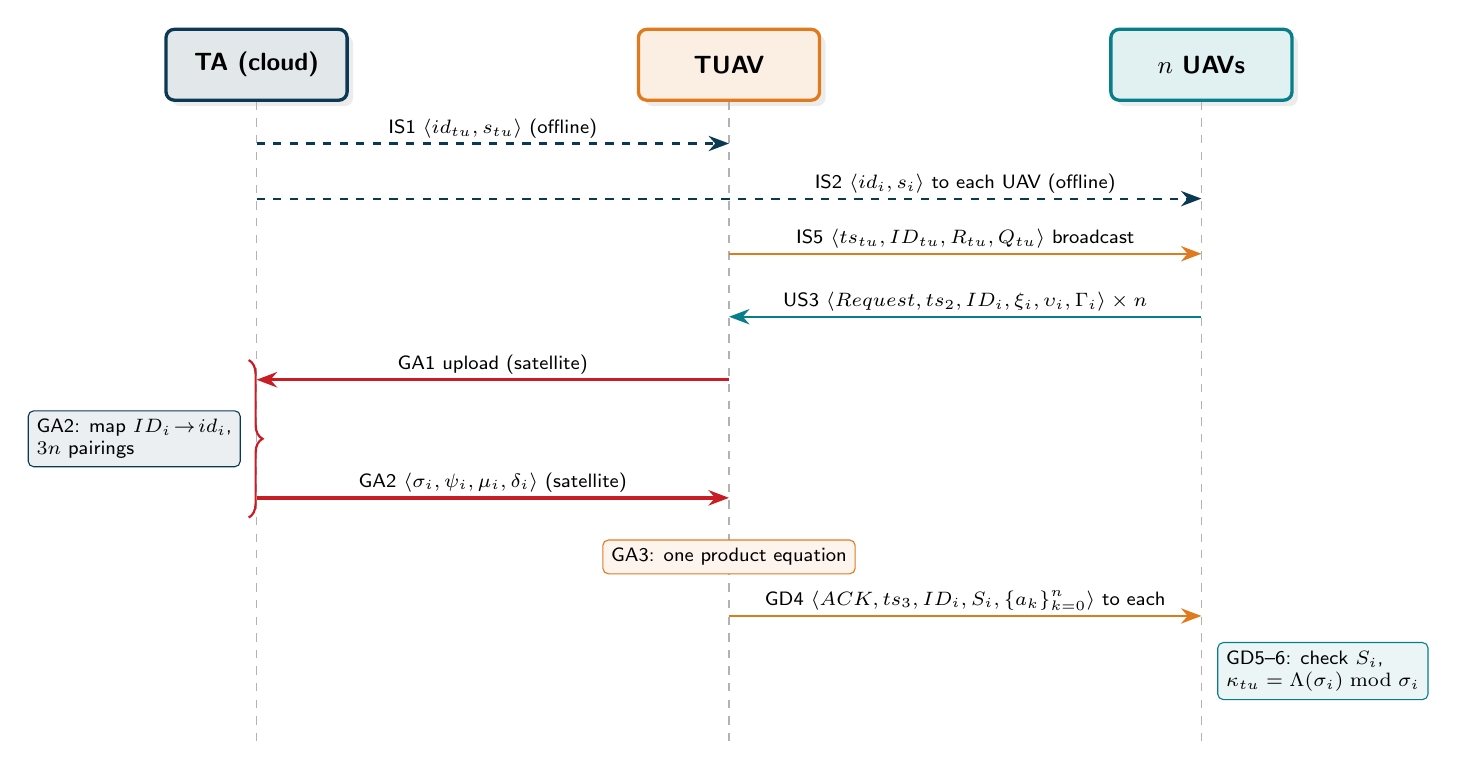
\begin{tikzpicture}[node distance=1cm]
  \node[ent=deep]  (ta)   at (0,0)   {TA (cloud)};
  \node[ent=hoc]   (tu)   at (6,0)   {TUAV};
  \node[ent=uavc]  (uav)  at (12,0)  {$n$ UAVs};
  \foreach \n in {ta,tu,uav}{ \draw[life] (\n.south) -- ++(0,-8.2); }
  \draw[msg=deep,dashed] (0,-1.0) -- node[lbl,above]{IS1 $\langle id_{tu},s_{tu}\rangle$ (offline)} (6,-1.0);
  \draw[msg=deep,dashed] (0,-1.7) -- node[lbl,above,pos=0.75]{IS2 $\langle id_i,s_i\rangle$ to each UAV (offline)} (12,-1.7);
  \draw[msg=hoc] (6,-2.4) -- node[lbl,above]{IS5 $\langle ts_{tu},ID_{tu},R_{tu},Q_{tu}\rangle$ broadcast} (12,-2.4);
  \draw[msg=uavc] (12,-3.2) -- node[lbl,above]{US3 $\langle Request,ts_2,ID_i,\xi_i,\upsilon_i,\Gamma_i\rangle\times n$} (6,-3.2);
  \draw[msg=bad,very thick] (6,-4.0) -- node[lbl,above]{GA1 upload (satellite)} (0,-4.0);
  \node[act=deep,anchor=east] at (-0.2,-4.75) {GA2: map $ID_i\!\to\! id_i$,\\ $3n$ pairings};
  \draw[msg=bad,very thick] (0,-5.5) -- node[lbl,above]{GA2 $\langle\sigma_i,\psi_i,\mu_i,\delta_i\rangle$ (satellite)} (6,-5.5);
  \node[act=hoc] at (6,-6.25) {GA3: one product equation};
  \draw[msg=hoc] (6,-7.0) -- node[lbl,above]{GD4 $\langle ACK,ts_3,ID_i,S_i,\{a_k\}_{k=0}^{n}\rangle$ to each} (12,-7.0);
  \node[act=uavc,anchor=west] at (12.2,-7.7) {GD5--6: check $S_i$,\\ $\kappa_{tu}=\Lambda(\sigma_i)\bmod\sigma_i$};
  \draw[bad,thick,decorate,decoration={brace,amplitude=5pt}] (-0.1,-3.75) -- (-0.1,-5.75);
\end{tikzpicture}}
\caption{Base scheme~\cite{base}. Red arrows cross the satellite link. GA3 cannot run until GA2 returns.}
\label{fig:base}
\end{figure}

\noindent The equations we use later (verbatim from~\cite{base}, Section~IV):
\begin{align}
  &\text{IS4:} && ID_{tu}=h_2(id_{tu},r_{tu}),\quad R_{tu}=r_{tu}\,h_2(ts_{tu},s_{tu})\in\mathbb{Z}_q,\quad Q_{tu}=s_{tu}\,h_2(ID_{tu},r_{tu})\,P \label{eq:is4}\\
  &\text{US1:} && \xi_i=h_1(r_i),\qquad ID_i=h_3(id_i,ts_2,\xi_i)\\
  &\text{US2:} && \upsilon_i=h_4(ID_i,ID_{tu},ts_2,\xi_i),\qquad
     \Gamma_i=\big[s_i\,h_3(ID_i,ts_2,s_i)\,R_{tu}-h_1(s_i\xi_i)\big]P-\upsilon_i\,h_1(r_i)\,Q_{tu} \label{eq:gamma}\\
  &\text{GA2:} && \sigma_i=h_1(s_i\xi_i)P,\ \ \psi_i=\hat e(\Gamma_i+\sigma_i,P),\ \ \mu_i=\hat e(h_3(ID_i,ts_2,s_i)P,s_iP),\ \ \delta_i=\hat e(s_{tu}P,\upsilon_i\xi_iP)\\
  &\text{GA3:} && \textstyle\prod_{i}\psi_i\,\big(\prod_i\delta_i\big)^{h_2(ID_{tu},r_{tu})}\overset{?}{=}\prod_i\mu_i^{R_{tu}}\label{eq:ga3}\\
  &\text{GD1--2:} && \omega_i=\textstyle\prod_{j\ne i}\sigma_j,\ \ \varphi_i\equiv\omega_i^{-1}\bmod\sigma_i,\ \
     \Lambda(x)=\kappa_{tu}\sum_{i=1}^{n}\omega_i\varphi_i+\prod_{i=1}^{n}(x-\sigma_i)=\sum_{k=0}^{n}a_kx^k \label{eq:lambda}\\
  &\text{GD6:} && \kappa_{tu}=\Lambda(\sigma_i)\bmod\sigma_i
\end{align}

% =====================================================================
\section{Critical Analysis of the Base Scheme}\label{sec:findings}
% =====================================================================
Each finding states \emph{what} fails, \emph{where} in the paper, \emph{why}, and the \emph{impact} on the paper's claims.
Where possible we confirmed the finding with a script; such cases are marked \emph{verified}.

% ---------------------------------------------------------------------
\subsection{Finding 1: the scheme is not infrastructure-less}
\begin{flawbox}[title={Authentication requires a live satellite link to the TA}]
\begin{finding}\label{f:online}
In Step GA1 the TUAV uploads every request to the TA. In Step GA2 the TA computes $\sigma_i,\psi_i,\mu_i,\delta_i$, which include all
pairings and need the secret $s_i$. The verification equation~\eqref{eq:ga3} of Step GA3 has no inputs other than these values. Nothing in the paper
gives a local fallback.
\end{finding}
\textbf{Why it matters.} The paper's own system model says the TA is reached through ``space networks'' (satellite), because the
terrestrial backhaul is destroyed. In the paper's scenario this link is shared, congested and possibly jammed. If $A$ is the probability that the
TA link is usable, the probability that an authentication round succeeds is exactly $A$. Its latency also includes one satellite round trip
(typically about 30--60\,ms for LEO and about 500--600\,ms for GEO).

\textbf{Impact.} When the link is lost, authentication does not slow down, it \emph{stops}. The dependency on infrastructure was not removed; it
was moved from a roadside pole to a satellite link that nobody in the field controls.
\end{flawbox}

% ---------------------------------------------------------------------
\subsection{Finding 2: the TA can impersonate every UAV}
Look again at Step US2, equation~\eqref{eq:gamma}. The last term uses $h_1(r_i)$, and Step US1 defined $\xi_i=h_1(r_i)$, which is sent in clear
in Step US3. Substituting gives
\begin{equation}
  \Gamma_i=\big[s_i\,h_3(ID_i,ts_2,s_i)\,R_{tu}-h_1(s_i\xi_i)\big]P-\upsilon_i\,\xi_i\,Q_{tu}.\label{eq:gamma2}
\end{equation}
Every quantity on the right is either the TA-issued secret $s_i$ or public ($ts_2,\xi_i,\upsilon_i,R_{tu},Q_{tu}$; $ID_i$ needs $id_i$, which
the TA also holds). The UAV's own random value $r_i$ enters only through $\xi_i$, and $\xi_i$ is public.

\begin{flawbox}[title={Key escrow and no non-repudiation (Table II claims F4 and F10 do not hold)}]
\begin{finding}\label{f:escrow}
The TA (or anyone who breaches it) can produce a valid request for any UAV $i$ in any session: choose $r_i$, compute
$\xi_i,ID_i,\upsilon_i$, then compute $\Gamma_i$ by~\eqref{eq:gamma2}. The request satisfies~\eqref{eq:ga3} for the same algebraic reason an honest one does.
\end{finding}
\textbf{Why.} In real certificateless cryptography~\cite{alriyami} a user's full private key combines a KGC-issued \emph{partial} key with a
\emph{secret value} the user picks and never reveals. Here the user's part ($r_i$) is effectively published, so only the TA-issued part remains.
The scheme is effectively a shared-key scheme with the TA, presented in pairing notation.

\textbf{Consequences.}
(i) \emph{Key escrow} (F4 \no): the TA can sign for any UAV. It also computes every $\sigma_i$ in GA2, so it can read the group key $\kappa_{tu}$.
(ii) \emph{Non-repudiation} (F10 \no): verification needs $\mu_i=\hat e(h_3(\cdot)P,s_iP)$, which only the holder of $s_i$ can compute. Any
credential could therefore have been produced by the TA, and a UAV can always deny it.
(iii) The pairings are not even necessary: the TA could check $\Gamma_i$ by recomputing~\eqref{eq:gamma2} with two scalar multiplications.
\end{flawbox}

% ---------------------------------------------------------------------
\subsection{Finding 3: no forward secrecy}
\begin{flawbox}[title={One leaked $s_i$ exposes every past group key (Table II claim F7 does not hold)}]
\begin{finding}\label{f:fs}
The decrypting key $\sigma_i=h_1(s_i\xi_i)P$ is a deterministic function of the long-term secret $s_i$ and the public $\xi_i$. An adversary that
records traffic and later learns $s_i$ (for example by capturing the UAV) recomputes $\sigma_i$ for every recorded session and then
$\kappa_{tu}=\Lambda(\sigma_i)\bmod\sigma_i$ from the recorded coefficients.
\end{finding}
\textbf{Why.} Forward secrecy needs an \emph{ephemeral} secret that is erased after the session, for example a Diffie--Hellman exponent. The scheme has none.
\end{flawbox}

% ---------------------------------------------------------------------
\subsection{Finding 4: the CRT group key leaks, and revocation fails}
\paragraph{(a) The construction is not well defined.}
Step GA2 defines $\sigma_i=h_1(s_i\xi_i)P$, an \emph{elliptic-curve point}. Step GD1 then multiplies points ($\omega_i=\prod_{j\ne i}\sigma_j$), inverts
modulo a point ($\varphi_i\equiv\omega_i^{-1}\bmod\sigma_i$), and Step GD6 reduces modulo a point. None of these operations is defined for points.
Under any reading that makes them work (for example $\sigma_i$ replaced by an integer derived from the point), the paper still omits three conditions
that correctness requires: the $\sigma_i$ must be pairwise coprime, $\kappa_{tu}<\min_i\sigma_i$, and~\eqref{eq:lambda} must be evaluated over the
integers, not modulo $q$.

\paragraph{(b) The polynomial reveals everyone's key.}
\begin{lemma}\label{lem:leak}
Let $C=\kappa_{tu}\sum_i\omega_i\varphi_i$. Then for every member $j$, \;$\Lambda(\sigma_j)=C$ \;and\; $\Lambda(x)-\Lambda(\sigma_j)=\prod_{i=1}^{n}(x-\sigma_i)$.
\end{lemma}
\begin{proof}
By~\eqref{eq:lambda}, $\Lambda(x)=C+\prod_i(x-\sigma_i)$ and the product vanishes at $x=\sigma_j$. Subtracting gives the second identity.
\end{proof}
So any member $j$ knows its own $\sigma_j$, computes the constant $\Lambda(\sigma_j)$, and obtains the monic integer polynomial $\prod_i(x-\sigma_i)$.
Its roots, which are the decrypting keys of \emph{all} members, can be found in polynomial time (integer root finding). Note also that the coefficients
$a_1,\dots,a_n$ are exactly the coefficients of $\prod_i(x-\sigma_i)$; only $a_0$ is masked.

\begin{flawbox}[title={A revoked UAV still obtains the new group key (verified)}]
\begin{finding}\label{f:crt}
In Step DU1 the TUAV builds $\Lambda^*(x)=\prod_{i\in S'}(x-\sigma_i)+\kappa^*_{tu}\sum_{i\in S'}\omega_i\varphi_i$ over the remaining set $S'$, and
\emph{reuses} the remaining members' old $\sigma_i$ (the paper presents this as an advantage). A member $k$ that is removed had already learned every
$\sigma_j$ through Lemma~\ref{lem:leak}. It picks any remaining $j\in S'$ and computes
\[
  \kappa^*_{tu}=\Lambda^*(\sigma_j)\bmod\sigma_j .
\]
\end{finding}
\textbf{Verification.} Our script \texttt{scripts/crt\_revocation\_attack.py} builds GD1--GD2 for $n=12$ members with 160-bit prime moduli, recovers
all twelve $\sigma_i$ from member~0's view, revokes two members, rebuilds $\Lambda^*$ by DU1, and checks the attack:
\begin{center}
\begin{tcolorbox}[colback=black!85,colframe=black!85,coltext=white,width=0.82\linewidth,arc=1mm,boxrule=0pt,fontupper=\ttfamily\small]
correctness holds for all 12 members\\
(A) insider recovered all sigma\_i: True\\
\hspace*{1.5em}revoked member's own sigma gives kappa*? False\\
(B) revoked member, using a stolen sigma, gets kappa*: True
\end{tcolorbox}
\end{center}
\textbf{Impact.} Group forward secrecy after revocation fails, and so does the claim of Theorem~5 that ``removed UAVs are locked out''. A UAV that joins
once and is then evicted keeps reading the group traffic.
\end{flawbox}

\begin{figure}[H]
\centering
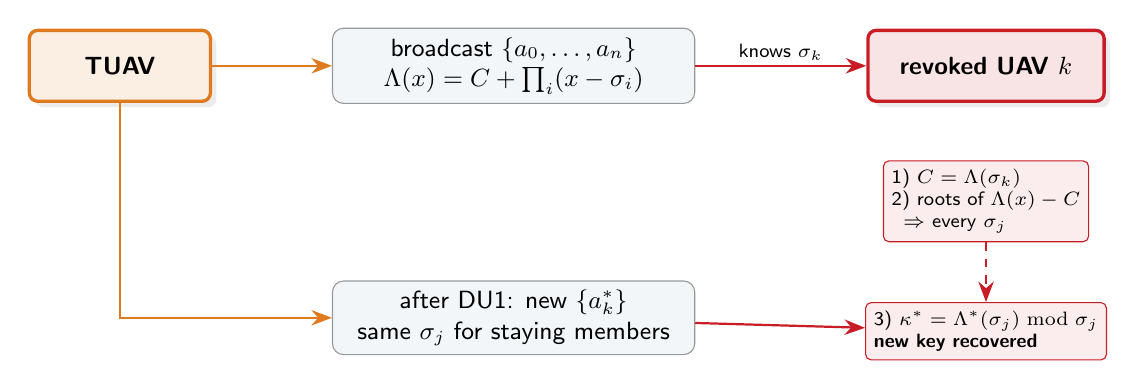
\begin{tikzpicture}[font=\sffamily\small]
  \node[ent=hoc] (tu) at (0,0) {TUAV};
  \node[draw=black!40,fill=soft,rounded corners,align=center,minimum width=4.6cm] (pub) at (5,0)
      {broadcast $\{a_0,\dots,a_n\}$\\ $\Lambda(x)=C+\prod_i(x-\sigma_i)$};
  \draw[msg=hoc] (tu) -- (pub);
  \node[ent=bad,minimum width=3cm] (k) at (11,0) {revoked UAV $k$};
  \draw[msg=bad] (pub) -- node[lbl,above]{knows $\sigma_k$} (k);
  \node[act=bad,anchor=north] (s1) at (11,-1.2) {1) $C=\Lambda(\sigma_k)$\\2) roots of $\Lambda(x)-C$\\ \;\;$\Rightarrow$ every $\sigma_j$};
  \node[draw=black!40,fill=soft,rounded corners,align=center,minimum width=4.6cm] (pub2) at (5,-3.2)
      {after DU1: new $\{a^*_k\}$\\ same $\sigma_j$ for staying members};
  \node[act=bad,anchor=north] (s2) at (11,-3.0) {3) $\kappa^*=\Lambda^*(\sigma_j)\bmod\sigma_j$\\ \textbf{new key recovered}};
  \draw[msg=hoc] (tu) |- (pub2);
  \draw[msg=bad] (pub2) -- (s2);
  \draw[msg=bad,dashed] (s1) -- (s2);
\end{tikzpicture}
\caption{Revocation break (Finding~\ref{f:crt}): an insider learns every decrypting key from the public coefficients and later uses a
staying member's key to open the updated polynomial.}
\label{fig:crtattack}
\end{figure}

\paragraph{(c) The real size of the broadcast.}
The coefficients $a_k$ are integers whose length grows with $n$ (they are products of up to $n$ 160-bit moduli). Table~V of~\cite{base} counts only
the request, $104n$ bytes. We computed the exact size of $\{a_k\}$ for random 160-bit prime moduli (Table~\ref{tab:crtsize}). Because Step GD3 sends
the acknowledgement ``one by one to each vehicle'', the total traffic is $n$ times larger again: $O(n^2)$ bits per ACK and $O(n^3)$ in total.

\begin{table}[H]
\centering\small
\caption{Measured size of the CRT coefficient set (\texttt{scripts/compute\_results.py}).}
\label{tab:crtsize}
\begin{tabular}{@{}rrrr@{}}
\toprule
$n$ & per ACK & all $n$ ACKs & paper's Table~V ($104n$) \\
\midrule
 20 &   4.1 KiB &  83.0 KiB &  2.0 KiB \\
 60 &  36.0 KiB &   2.11 MiB &  6.1 KiB \\
120 & 142.7 KiB &  16.72 MiB & 12.2 KiB \\
\bottomrule
\end{tabular}
\end{table}

% ---------------------------------------------------------------------
\subsection{Finding 5: the unforgeability proof is empty}
\begin{flawbox}[title={Theorem 1 reduces to a problem that is not hard}]
\begin{finding}\label{f:proof}
The proof of Theorem~1 embeds the CDH instance $(aP,bP)=\big(s_{tu}P,\ (\sum_i\upsilon_i\xi_i)P\big)$. But $\upsilon_i$ and $\xi_i$ are sent in clear in
every request, so $b=\sum_i\upsilon_i\xi_i$ is public and $abP=b\cdot(s_{tu}P)$ can be computed directly. Solving this ``instance'' is
not hard, so the reduction proves nothing.
\end{finding}
\textbf{Further gaps.} (i) The reduction is built around the TUAV's secret $s_{tu}$, whereas forging a \emph{UAV's} credential should depend on that
UAV's secret. (ii) Theorems~2--5 are argued only in words. (iii) The batch check~\eqref{eq:ga3} uses no random small exponents~\cite{bgr}. Because
$\prod_i\psi_i=\hat e\big(\sum_i(\Gamma_i+\sigma_i),P\big)$, replacing $\Gamma_1,\Gamma_2$ by $\Gamma_1+\Delta,\ \Gamma_2-\Delta$ leaves the batch valid
although both individual credentials are now invalid. (iv) Step GA4 has no else-branch, so a single bad request rejects the whole batch and the
culprit cannot be identified.
\end{flawbox}

% ---------------------------------------------------------------------
\subsection{Finding 6: the cost accounting leaves out the expensive part}\label{sec:f6}
\begin{flawbox}[title={The reported 151\,ms excludes the TA's pairings (and the satellite delay)}]
\begin{finding}\label{f:cost}
Section VI-A states that ``the computation overhead on the TUAV side is considered'' for GA. However, Step GA2 performs, per UAV, three pairings
($\psi_i,\mu_i,\delta_i$), three scalar multiplications in $\G_1$ and one point addition:
\[ T_{\TA}=3T_P+3T_{SM\text{-}P}+T_{PA\text{-}P}+2T_{SH}=29.7414\ \text{ms per UAV.} \]
\end{finding}
In addition, $\Gamma_i$ is costed in the 160-bit group $\G$ ($T_{SM\text{-}E}$), but GA2 pairs it, so it must live in the pairing group $\G_1$.
Correcting both (constants from~\cite{base}):
\begin{center}\small
\begin{tabular}{@{}lccc@{}}
\toprule
Quantity & reported in~\cite{base} & honest accounting & ratio\\
\midrule
UAV signing (US) & 1.8203 ms & 5.3970 ms ($\Gamma_i\in\G_1$) & $3.0\times$\\
Single verification (SA) & 2.1578 ms & 31.8992 ms + RTT & $14.8\times$\\
Group auth.\ $n{=}120$ (GA) & 151.19 ms & 3720.16 ms + RTT & $24.6\times$\\
Request size & 104 B & 192 B ($\Gamma_i\in\G_1$, 128 B) & $1.8\times$\\
Satellite traffic per UAV & not reported & 192 B up + 512 B down & --\\
Key ACK, $n{=}120$ & not reported & 142.7 KiB each & --\\
\bottomrule
\end{tabular}
\end{center}
\textbf{Impact.} With honest accounting the base scheme is the \emph{slowest} of the five schemes it compares (Mei 696\,ms, Kumar 1985\,ms, Ali 333\,ms,
Xu 1668\,ms at $n{=}120$), and it is the only one that needs a wide-area round trip.
\end{flawbox}

% ---------------------------------------------------------------------
\subsection{Summary of findings}
\begin{table}[H]
\centering\small
\caption{Our findings mapped to the base paper's claims.}
\label{tab:findings}
\begin{tabularx}{\linewidth}{@{}c>{\raggedright\arraybackslash}X l l c@{}}
\toprule
\# & What fails & Where & Claim affected & Verified\\
\midrule
1 & Authentication needs a live satellite link to the TA & GA1--GA3 & ``infrastructure-less'' & by inspection\\
2 & TA can forge any UAV; verification needs $s_i$ & US2, GA2 & F4, F10 & algebraic\\
3 & Past group keys recoverable from $s_i$ & GA2, GD6 & F7 & algebraic\\
4 & Every member learns all $\sigma_i$; revoked UAV gets new key & GD2, DU1 & F3, F5, Thm 5 & script\\
5 & Theorem 1's reduction is empty; batch check unsound; no failure branch & Thm 1, GA3--4 & F1, F8 & algebraic\\
6 & TA pairings and satellite RTT omitted; $\Gamma_i$ in wrong group & Sec. VI & Tables III--V & recomputed\\
\bottomrule
\end{tabularx}
\end{table}

\begin{keybox}
All six findings share one root cause: \textbf{the TA is inside every operation}. It holds every secret, performs every check, and is reachable only over the
link the disaster degrades. Removing the TA from the field is therefore the central design goal of our framework.
\end{keybox}

% =====================================================================
\section{System Model, Threat Model and Design Goals}\label{sec:model}
% =====================================================================

\subsection{System model}
We keep the base paper's scenario: RSUs are destroyed, and an ECRV with its TUAV is deployed. We extend it in two directions: vehicles become
first-class participants, and \emph{several} TUAVs cover neighbouring cells (Figure~\ref{fig:arch}).

\begin{figure}[H]
\centering
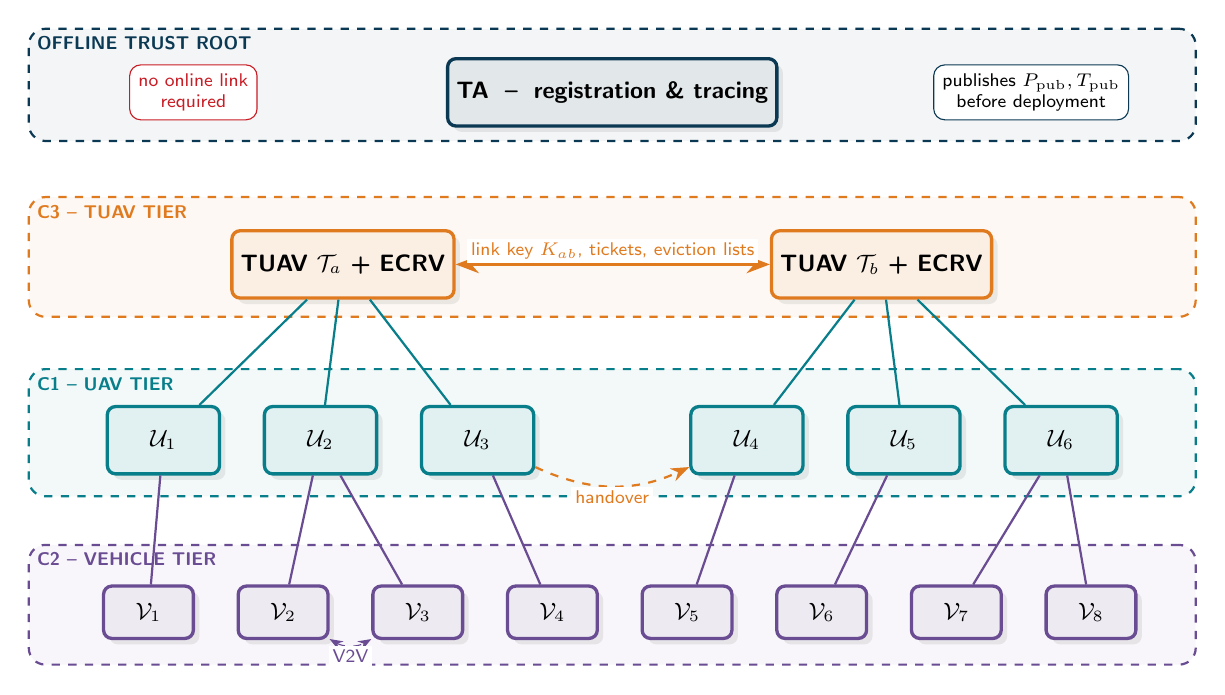
\begin{tikzpicture}[font=\sffamily\small,scale=0.95,transform shape]
  % tiers
  \node[tier=deep,minimum width=15.6cm,minimum height=1.5cm] (t0) at (0,4.3) {};
  \node[anchor=north west,font=\sffamily\scriptsize\bfseries,text=deep] at (t0.north west) {OFFLINE TRUST ROOT};
  \node[ent=deep,minimum width=4cm] (ta) at (0,4.2) {TA \;--\; registration \& tracing};
  \node[draw=deep,fill=white,rounded corners,font=\scriptsize\sffamily,align=center] at (5.6,4.2) {publishes $\Ppub,\Tpub$\\ before deployment};
  \node[draw=bad,fill=white,rounded corners,font=\scriptsize\sffamily,align=center,text=bad] at (-5.6,4.2) {no online link\\ required};

  \node[tier=hoc,minimum width=15.6cm,minimum height=1.6cm] (t3) at (0,2.0) {};
  \node[anchor=north west,font=\sffamily\scriptsize\bfseries,text=hoc] at (t3.north west) {C3 -- TUAV TIER};
  \node[ent=hoc] (ta1) at (-3.6,1.9) {TUAV $\Ta$ + ECRV};
  \node[ent=hoc] (tb1) at (3.6,1.9) {TUAV $\Tb$ + ECRV};
  \draw[{Stealth}-{Stealth},very thick,hoc] (ta1) -- node[lbl,above]{link key $K_{ab}$, tickets, eviction lists} (tb1);

  \node[tier=uavc,minimum width=15.6cm,minimum height=1.7cm] (t1) at (0,-0.35) {};
  \node[anchor=north west,font=\sffamily\scriptsize\bfseries,text=uavc] at (t1.north west) {C1 -- UAV TIER};
  \foreach \x/\l in {-6/1,-3.9/2,-1.8/3}{ \node[ent=uavc,minimum width=1.5cm] (u\l) at (\x,-0.45) {$\U_{\l}$}; }
  \foreach \x/\l in {1.8/4,3.9/5,6/6}{ \node[ent=uavc,minimum width=1.5cm] (u\l) at (\x,-0.45) {$\U_{\l}$}; }
  \foreach \l in {1,2,3}{ \draw[uavc,thick] (ta1) -- (u\l); }
  \foreach \l in {4,5,6}{ \draw[uavc,thick] (tb1) -- (u\l); }
  \draw[-{Stealth},thick,hoc,dashed] (u3) to[bend right=25] node[lbl,below]{handover} (u4);

  \node[tier=vehc,minimum width=15.6cm,minimum height=1.6cm] (t2) at (0,-2.65) {};
  \node[anchor=north west,font=\sffamily\scriptsize\bfseries,text=vehc] at (t2.north west) {C2 -- VEHICLE TIER};
  \foreach \x/\l in {-6.2/1,-4.4/2,-2.6/3,-0.8/4,1.0/5,2.8/6,4.6/7,6.4/8}{ \node[ent=vehc,minimum width=1.2cm,minimum height=0.7cm] (v\l) at (\x,-2.75) {$\V_{\l}$}; }
  \draw[vehc,thick] (u1) -- (v1); \draw[vehc,thick] (u2) -- (v2); \draw[vehc,thick] (u2) -- (v3);
  \draw[vehc,thick] (u3) -- (v4); \draw[vehc,thick] (u4) -- (v5); \draw[vehc,thick] (u5) -- (v6); \draw[vehc,thick] (u6) -- (v7); \draw[vehc,thick] (u6) -- (v8);
  \draw[{Stealth}-{Stealth},vehc,dashed] (v2) to[bend right=30] node[lbl,below]{V2V} (v3);
\end{tikzpicture}
\caption{The three-tier framework. The TA (top) acts only before deployment and for later tracing; all field operations (C1--C3) run without it.}
\label{fig:arch}
\end{figure}

\begin{itemize}
  \item \textbf{\textcolor{deep}{Trusted Authority $\TA$}}: generates system parameters, registers every entity \emph{before} deployment, and can
        later trace a pseudonym to a real identity. It is \emph{not} assumed reachable during operation.
  \item \textbf{\textcolor{hoc}{TUAV $\Ta$}}: the cell controller (powered by its ECRV). It verifies UAVs and vehicles, distributes keys, and talks to
        neighbouring TUAVs. TUAVs have fixed public identities $\ID_a$; they are infrastructure, not users, so they need no anonymity.
  \item \textbf{\textcolor{uavc}{UAVs $\U_i$}}: battery-powered and resource-limited. They form the aerial relay layer.
  \item \textbf{\textcolor{vehc}{Vehicles $\V_j$}}: hold the same kind of credential as UAVs, reach a TUAV through a UAV or directly, and communicate V2V.
\end{itemize}

\subsection{Threat model}
\begin{itemize}
  \item \textbf{Network adversary} (Dolev--Yao~\cite{dolevyao}): reads, drops, replays, modifies and injects messages on every wireless link.
  \item \textbf{Type-I adversary}~\cite{alriyami}: an outsider who may \emph{replace} any entity's public key but does not know the TA master key $s$.
  \item \textbf{Type-II adversary}: an honest-but-curious (or breached) TA that knows $s$ and all partial keys but not an entity's secret value $x$.
        This is the adversary under which the base scheme fails (Finding~\ref{f:escrow}).
  \item \textbf{Insiders}: compromised or revoked UAVs and vehicles that know their own keys and every group key they ever legitimately received.
  \item \textbf{Batch poisoner}: injects requests with invalid signatures so that batches fail (denial of service).
\end{itemize}
\textbf{Trust assumptions.} TUAVs are trusted to run the protocol honestly; a \emph{captured} TUAV is discussed as a limitation
(Section~\ref{sec:discussion}). Clocks are loosely synchronised (GNSS) for timestamp checks. Hash functions are modelled as random oracles.

\subsection{Design goals}
\begin{center}\small
\begin{tabularx}{\linewidth}{@{}l>{\raggedright\arraybackslash}X l@{}}
\toprule
Goal & Meaning & Fixes\\
\midrule
G1 Authority independence & No field operation (C1--C3) waits for the TA & Finding 1\\
G2 Escrow-freeness & The TA cannot sign for, or derive the keys of, any registered entity & Finding 2\\
G3 Unforgeability \& non-repudiation & Publicly verifiable signatures under ECDLP, with a valid proof sketch & Findings 2, 5\\
G4 Conditional privacy & Pseudonyms that cannot be linked across epochs; only the TA can trace them, offline & (kept)\\
G5 Key secrecy & Forward secrecy against long-term key loss; leavers cannot read new keys, joiners cannot read old ones & Findings 3, 4\\
G6 Robust batching & Sound batch test; bounded cost when a batch fails & Finding 5\\
G7 Coverage & Vehicles included; seamless handover between TUAVs & new\\
G8 Efficiency & Comparable cost to the base scheme under the same constants, linear traffic & Finding 6\\
\bottomrule
\end{tabularx}
\end{center}

% =====================================================================
\section{Preliminaries and Notation}\label{sec:prelim}
% =====================================================================
\paragraph{Elliptic-curve group.} $\G$ is a cyclic group of prime order $q$ on an elliptic curve with generator $P$. We need no pairing.
\begin{definition}[ECDLP]
Given $(P,aP)$ with $a\in\Zq$, computing $a$ is infeasible for any probabilistic polynomial-time (PPT) algorithm.
\end{definition}
\begin{definition}[CDH]
Given $(P,aP,bP)$, computing $abP$ is infeasible for any PPT algorithm.
\end{definition}

\paragraph{Schnorr-type signature.} A signer with key $z$ and public key $Z=zP$ picks $r$, sets $R=rP$, $c=H(m,R,\dots)$, $v=r+cz$; the verifier checks
$vP=R+cZ$. Unforgeability reduces to ECDLP in the random-oracle model via the forking lemma~\cite{schnorr,forking}.

\paragraph{Certificateless keys~\cite{alriyami}.} A full private key combines a KGC-issued \emph{partial key} with a \emph{secret value} chosen by the user,
so neither the KGC alone nor a key-replacing outsider can sign. Pairing-free certificateless signatures of this kind are well studied; ECLAS~\cite{eclas}
(reference~[34] of the base paper) is one example.

\paragraph{Small-exponent batch test~\cite{bgr}.} To check $n$ equations $v_iP=R_i+c_i\pk_i$ at once, the verifier draws random
$\lambda_i\in[1,2^{\ell_\lambda}]$ and checks one weighted sum. An invalid batch passes with probability at most $2^{-\ell_\lambda}$.

\paragraph{Symmetric tools.} $\KDF$ is HKDF~\cite{hkdf}; $(\Enc,\Dec)$ is an authenticated encryption scheme with associated data (AES-128-GCM~\cite{gcm});
$\MAC$ is HMAC-SHA-256. $\Enc(K,m;\,\mathit{AD})$ encrypts $m$ and authenticates both $m$ and the associated data $\mathit{AD}$.

\begin{table}[H]
\centering\small
\caption{Notation of the proposed framework (our symbols).}
\label{tab:notation}
\begin{tabularx}{\linewidth}{@{}l>{\raggedright\arraybackslash}X@{}}
\toprule
Symbol & Meaning\\
\midrule
$\TA,\ \Ta,\ \U_i,\ \V_j,\ \Ent,\ \M$ & Trusted Authority; TUAV of cell $a$; UAV $i$; vehicle $j$; any entity; a moving member\\
$\G,\ q,\ P$ & elliptic-curve group, its prime order, generator\\
$s,\ \Ppub=sP$ & TA master key (signs partial keys) and its public key\\
$t,\ \Tpub=tP$ & TA tracing key (opens pseudonyms) and its public key\\
$\RID_\Ent$ & real identity of entity $\Ent$ (never transmitted)\\
$\ep,\ \PID_\Ent=(\PID^1_\Ent,\PID^2_\Ent)$ & epoch index; pseudonym of $\Ent$ valid only in epoch $\ep$\\
$x_\Ent,\ X_\Ent=x_\Ent P$ & secret value chosen by $\Ent$ (TA never sees $x_\Ent$) and its public part\\
$y_\Ent,\ Y_\Ent,\ d_\Ent$ & TA nonce, its public part $Y_\Ent=y_\Ent P$, and the partial private key\\
$h_\Ent=\Ho(\PID_\Ent,\ep,X_\Ent,Y_\Ent)$ & binding hash of the credential\\
$\sk_\Ent=x_\Ent+d_\Ent,\ \pk_\Ent=X_\Ent+Y_\Ent+h_\Ent\Ppub$ & full private key; full public key ($\sk_\Ent P=\pk_\Ent$)\\
$(R,v)$, $c$ & signature, $R=rP$, $v=r+c\,\sk$; challenge $c=\Ht(\cdot)$\\
$\lambda_i,\ \ell_\lambda$ & random batch weights, $\lambda_i\in[1,2^{\ell_\lambda}]$, $\ell_\lambda=64$\\
$e_\Ent,\ E_\Ent=e_\Ent P$ & ephemeral Diffie--Hellman secret and public value (erased after use)\\
$K_i$ & pairwise key between $\Ta$ and member $i$\\
$\GK_a,\ \VK_a,\ \nu$ & UAV group key, vehicle regional key of cell $a$, key version\\
$K_{ab}$ & link key between neighbouring TUAVs $\Ta,\Tb$\\
$\Tk_\M,\ \hk_\M,\ N_\M,\ \mathit{exp}$ & handover ticket, handover key, ticket nonce, ticket expiry\\
$\ts,\ \Delta t$ & timestamp, acceptance window\\
$\mathcal{L}$ & eviction/revocation list (hashes of banned pseudonyms)\\
$\Hz:\G\times\{0,1\}^*\!\to\!\{0,1\}^{|\RID|}$, $\Ho,\Ht:\{0,1\}^*\!\to\!\Zq$, $\Hd$ & hash functions ($\Hd$: SHA-256, used for list indices)\\
$\cat$ & concatenation\\
\bottomrule
\end{tabularx}
\end{table}

% =====================================================================
\section{Proposed Framework: Setup and Offline Registration}\label{sec:setup}
% =====================================================================
The framework has five phases (Figure~\ref{fig:phases}). Only Phase~0 involves the TA; Phases~1--3 run in the field without it; Phase~4 is optional
and happens whenever the TA becomes reachable, without blocking anything.

\begin{figure}[H]
\centering
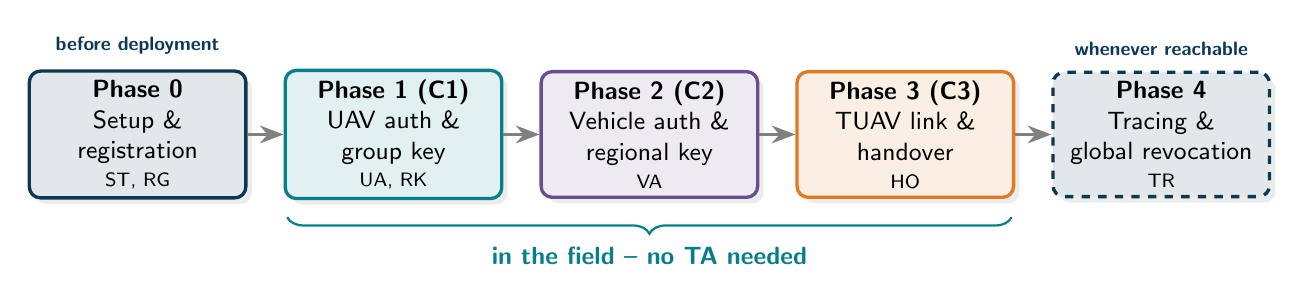
\begin{tikzpicture}[font=\sffamily\small,
  ph/.style={draw=#1,fill=#1!12,very thick,rounded corners=4pt,minimum width=2.75cm,minimum height=1.55cm,align=center,drop shadow={opacity=0.15}}]
  \node[ph=deep] (p0) at (0,0)   {\textbf{Phase 0}\\Setup \&\\registration\\[-1pt]{\scriptsize ST, RG}};
  \node[ph=uavc] (p1) at (3.25,0) {\textbf{Phase 1 (C1)}\\UAV auth \&\\group key\\[-1pt]{\scriptsize UA, RK}};
  \node[ph=vehc] (p2) at (6.5,0) {\textbf{Phase 2 (C2)}\\Vehicle auth \&\\regional key\\[-1pt]{\scriptsize VA}};
  \node[ph=hoc]  (p3) at (9.75,0) {\textbf{Phase 3 (C3)}\\TUAV link \&\\handover\\[-1pt]{\scriptsize HO}};
  \node[ph=deep,dashed] (p4) at (13,0) {\textbf{Phase 4}\\Tracing \&\\global revocation\\[-1pt]{\scriptsize TR}};
  \foreach \a/\b in {p0/p1,p1/p2,p2/p3,p3/p4}{ \draw[-{Stealth[length=3mm]},very thick,black!50] (\a) -- (\b); }
  \draw[decorate,decoration={brace,amplitude=6pt,mirror},thick,uavc] (1.9,-1.05) -- node[below=7pt,text=uavc]{\textbf{in the field -- no TA needed}} (11.1,-1.05);
  \node[above=2pt of p0,font=\scriptsize\sffamily\bfseries,text=deep] {before deployment};
  \node[above=2pt of p4,font=\scriptsize\sffamily\bfseries,text=deep] {whenever reachable};
\end{tikzpicture}
\caption{Phases of the framework and their step labels.}
\label{fig:phases}
\end{figure}

\subsection{System setup (ST)}
\begin{stepbox}{deep}{ST1--ST2 \;(TA, once)}
\steplabel{deep}{ST1.} $\TA$ chooses $(\G,q,P)$, the master key $s\in\Zq$ and the tracing key $t\in\Zq$, and sets $\Ppub=sP$, $\Tpub=tP$.\\
\steplabel{deep}{ST2.} $\TA$ publishes $\mathit{params}=\langle \G,q,P,\Ppub,\Tpub,\Hz,\Ho,\Ht,\Hd,\KDF,\Enc,\MAC\rangle$ and keeps $(s,t)$ secret.
\end{stepbox}
\begin{whybox}
Two separate TA keys give \emph{separation of duties}. $s$ certifies keys and $t$ opens pseudonyms, so the two can be held by different offices
(for example, the network operator and the law-enforcement agency). Leaking one does not give the power of the other.
\end{whybox}

\subsection{Entity registration (RG)}
Every UAV, vehicle and TUAV registers once, over a secure channel, before deployment. A mission is divided into $m$ \emph{epochs}
(for example 15 minutes each), and an entity receives one pseudonym credential per epoch.

\begin{stepbox}{deep}{RG1--RG4 \;(entity $\Ent$ $\leftrightarrow$ TA, offline)}
\steplabel{deep}{RG1.} For each epoch $\ep=1..m$, $\Ent$ picks a secret value $x^{(\ep)}_\Ent\in\Zq$ and computes $X^{(\ep)}_\Ent=x^{(\ep)}_\Ent P$.
It sends $\RID_\Ent$ and $\{X^{(\ep)}_\Ent\}$ to $\TA$, together with a Schnorr signature under each $x^{(\ep)}_\Ent$ on $\RID_\Ent\cat X^{(\ep)}_\Ent$
(proof of possession). \textbf{The values $x^{(\ep)}_\Ent$ never leave the entity.}\\[2pt]
\steplabel{deep}{RG2.} For each $\ep$, $\TA$ picks $\rho,y\in\Zq$ and computes
\[
 \PID^1=\rho P,\qquad \PID^2=\RID_\Ent\oplus\Hz(\rho\,\Tpub\cat\ep),\qquad Y=yP,
\]
\[
 h=\Ho(\PID,\ep,X^{(\ep)}_\Ent,Y),\qquad d=y+s\,h \bmod q .
\]
$\TA$ stores $(\RID_\Ent,\{\PID^{(\ep)}\})$ and the signed RG1 record, then erases $\rho,y$.\\[2pt]
\steplabel{deep}{RG3.} $\TA\to\Ent$: $\{(\PID^{(\ep)},Y^{(\ep)},d^{(\ep)})\}_{\ep=1}^{m}$.\\[2pt]
\steplabel{deep}{RG4.} $\Ent$ checks $d^{(\ep)}P\overset{?}{=}Y^{(\ep)}+h^{(\ep)}\Ppub$ for every $\ep$, and stores the credentials.
\end{stepbox}
\noindent A TUAV registers in the same way with its fixed public identity $\ID_a$ in place of a pseudonym and a single credential
$(X_a,Y_a,d_a)$, $h_a=\Ho(\ID_a,0,X_a,Y_a)$.

\paragraph{Correctness of the keys.} With $\sk=x+d$ and $\pk=X+Y+h\Ppub$:\;
$\sk\cdot P=xP+(y+sh)P=X+Y+h\Ppub=\pk$.
\emph{From here on, inside one epoch we write $x_\Ent,X_\Ent,\PID_\Ent,Y_\Ent,d_\Ent,h_\Ent$ without the superscript.}

\begin{whatbox}
Each entity ends up with a full key pair $(\sk_\Ent,\pk_\Ent)$ per epoch. The TA certified half of it ($d_\Ent$) but never saw the other half ($x_\Ent$).
Anyone holding only $\Ppub$ can check that $\pk_\Ent$ was certified, because $\pk_\Ent$ contains $h_\Ent\Ppub$.
\end{whatbox}
\begin{whybox}
\begin{itemize}[leftmargin=*]
  \item \textbf{Escrow-free (fixes Finding~\ref{f:escrow}).} Signing needs $\sk=x+d$. The TA knows $d$ but not $x$, so it cannot sign for $\Ent$.
  \item \textbf{No certificates.} The binding hash $h=\Ho(\PID,\ep,X,Y)$ ties the TA's signature to this exact $X$. An outsider who replaces $X$ changes
        $h$, and then needs a new $d$, which requires $s$.
  \item \textbf{Fresh $x^{(\ep)}$ per epoch.} If $X$ were the same in every epoch it would link the pseudonyms together. Per-epoch values keep epochs unlinkable.
  \item \textbf{Pseudonym = ElGamal-style encryption of $\RID$ under $\Tpub$.} Only the holder of $t$ can open it ($\rho\Tpub=t\,\PID^1$).
  \item \textbf{Proof of possession and the signed record.} A TA cannot later claim that an entity owns a key it does not, which supports non-repudiation in disputes.
\end{itemize}
\end{whybox}

% =====================================================================
\section{C1: Autonomous UAV Authentication and Group Key Management}\label{sec:c1}
% =====================================================================
\begin{keybox}
The TUAV verifies all requesting UAVs \emph{itself}, using only $\Ppub$, in one small-exponent batch. Each verified UAV receives the
group key encrypted under its own fresh Diffie--Hellman key. No satellite link, no pairings, no CRT polynomial.
\end{keybox}

\begin{figure}[H]
\centering
\resizebox{\linewidth}{!}{%
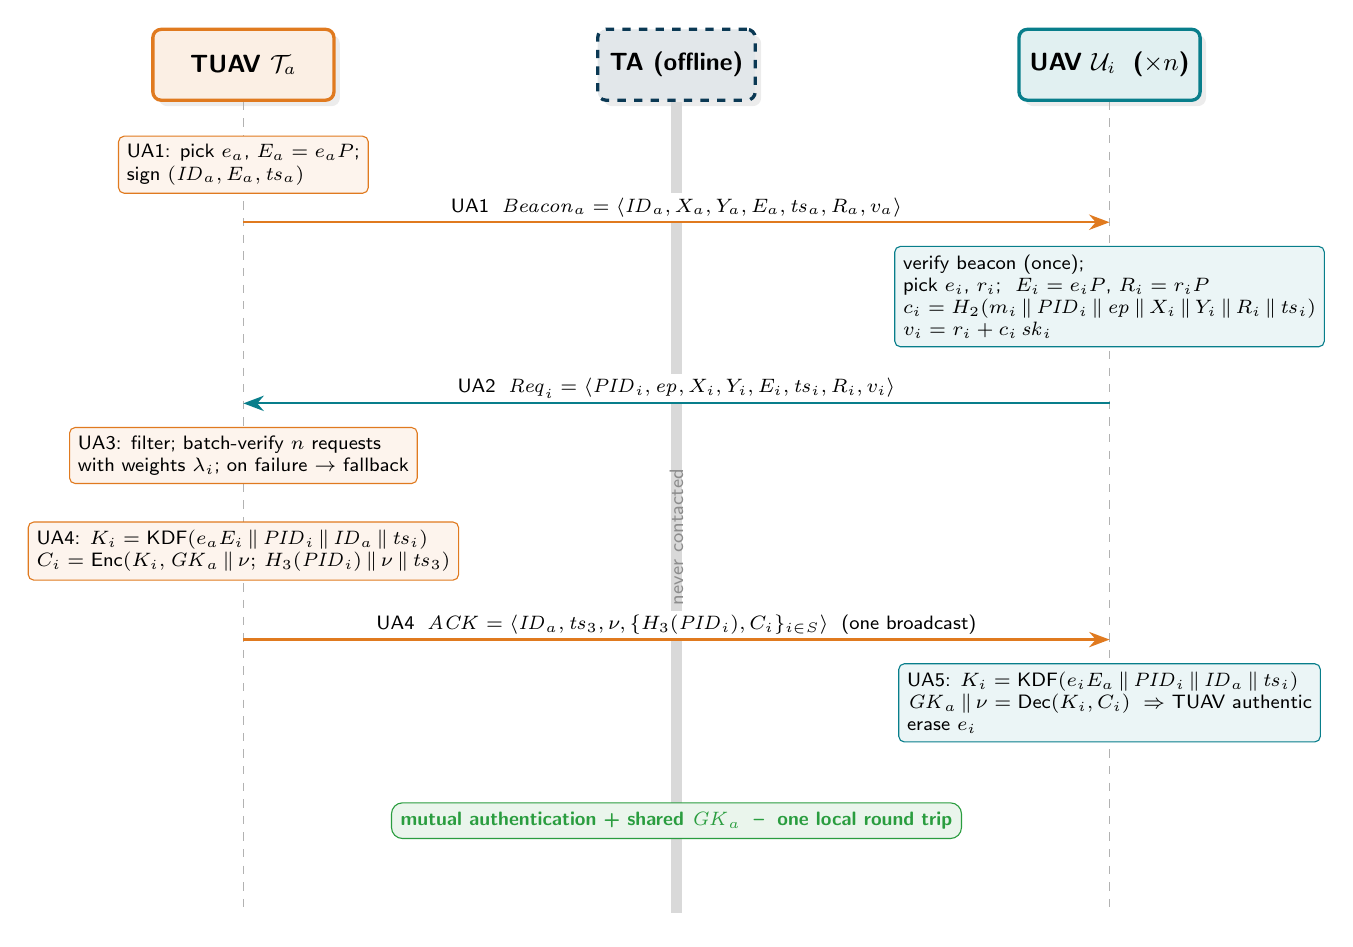
\begin{tikzpicture}[font=\sffamily\small]
  \node[ent=hoc]  (t) at (0,0)  {TUAV $\Ta$};
  \node[ent=uavc] (u) at (11,0) {UAV $\U_i$ \;($\times n$)};
  \node[ent=deep,dashed,minimum width=2cm] (ta) at (5.5,0) {TA (offline)};
  \draw[life] (t.south) -- ++(0,-10.3);  \draw[life] (u.south) -- ++(0,-10.3);
  \draw[black!15,line width=4pt] (ta.south) -- ++(0,-10.3);
  \node[font=\scriptsize\sffamily,text=black!45,rotate=90] at (5.5,-6) {never contacted};

  \node[act=hoc,anchor=north] at (0,-0.9) {UA1: pick $e_a$, $E_a=e_aP$;\\ sign $(\ID_a,E_a,\ts_a)$};
  \draw[msg=hoc] (0,-2.0) -- node[lbl,above]{UA1 \;$\mathit{Beacon}_a=\langle \ID_a,X_a,Y_a,E_a,\ts_a,R_a,v_a\rangle$} (11,-2.0);
  \node[act=uavc,anchor=north] at (11,-2.3) {verify beacon (once);\\ pick $e_i$, $r_i$;\ \ $E_i=e_iP$, $R_i=r_iP$\\ $c_i=\Ht(m_i\cat\PID_i\cat\ep\cat X_i\cat Y_i\cat R_i\cat\ts_i)$\\ $v_i=r_i+c_i\,\sk_i$};
  \draw[msg=uavc] (11,-4.3) -- node[lbl,above]{UA2 \;$\mathit{Req}_i=\langle \PID_i,\ep,X_i,Y_i,E_i,\ts_i,R_i,v_i\rangle$} (0,-4.3);
  \node[act=hoc,anchor=north] at (0,-4.6) {UA3: filter; batch-verify $n$ requests\\ with weights $\lambda_i$; on failure $\to$ fallback};
  \node[act=hoc,anchor=north] at (0,-5.8) {UA4: $K_i=\KDF(e_aE_i\cat\PID_i\cat\ID_a\cat\ts_i)$\\ $C_i=\Enc(K_i,\GK_a\cat\nu;\,\Hd(\PID_i)\cat\nu\cat\ts_3)$};
  \draw[msg=hoc] (0,-7.3) -- node[lbl,above]{UA4 \;$\mathit{ACK}=\langle \ID_a,\ts_3,\nu,\{\Hd(\PID_i),C_i\}_{i\in S}\rangle$ \;(one broadcast)} (11,-7.3);
  \node[act=uavc,anchor=north] at (11,-7.6) {UA5: $K_i=\KDF(e_iE_a\cat\PID_i\cat\ID_a\cat\ts_i)$\\ $\GK_a\cat\nu=\Dec(K_i,C_i)$ \;$\Rightarrow$ TUAV authentic\\ erase $e_i$};
  \node[draw=good,fill=good!10,rounded corners,font=\scriptsize\sffamily\bfseries,text=good] at (5.5,-9.6) {mutual authentication + shared $\GK_a$ \;--\; one local round trip};
\end{tikzpicture}}
\caption{C1 message flow. Compare with Figure~\ref{fig:base}: the satellite round trip and the TA's pairings are gone.}
\label{fig:c1}
\end{figure}

\subsection{Steps}
Let $m_i=(\texttt{"join"}\cat\ID_a\cat E_a\cat E_i)$ be the content a UAV signs; the TUAV can rebuild $m_i$ from the request and its own beacon.

\begin{stepbox}{uavc}{UA1 \;Beacon (TUAV, periodic)}
$\Ta$ picks a fresh $e_a\in\Zq$, sets $E_a=e_aP$, signs $(\ID_a\cat E_a\cat\ts_a)$ with $\sk_a$ to obtain $(R_a,v_a)$, and broadcasts
$\mathit{Beacon}_a=\langle\ID_a,X_a,Y_a,E_a,\ts_a,R_a,v_a\rangle$. A new $e_a$ is drawn every beacon period, and the old one is erased when the period ends.
\end{stepbox}

\begin{stepbox}{uavc}{UA2 \;Signed join request (each UAV)}
$\U_i$ checks $|\ts_a-\ts_{\mathrm{now}}|\le\Delta t$ and verifies the beacon once: $v_aP\overset{?}{=}R_a+c_a\,\pk_a$.
It picks $e_i,r_i\in\Zq$, computes $E_i=e_iP$, $R_i=r_iP$,
\[
  c_i=\Ht(m_i\cat\PID_i\cat\ep\cat X_i\cat Y_i\cat R_i\cat\ts_i),\qquad v_i=r_i+c_i\,\sk_i \bmod q,
\]
and sends $\mathit{Req}_i=\langle\PID_i,\ep,X_i,Y_i,E_i,\ts_i,R_i,v_i\rangle$.
\textbf{Cost: two scalar multiplications} (plus one beacon verification per beacon period).
\end{stepbox}

\begin{stepbox}{uavc}{UA3 \;Local batch verification with bounded fallback (TUAV)}
\textbf{Filter.} Collect the requests of one window. Drop any request whose timestamp is stale, whose $\ep$ is not current, whose $\Hd(\PID_i)\in\mathcal{L}$,
or whose $\PID_i$ already sent a request in this window.\\[2pt]
\textbf{Batch test.} Compute $h_i=\Ho(\PID_i,\ep,X_i,Y_i)$ and $c_i$, draw $\lambda_i\in[1,2^{64}]$, and check
\begin{equation}
  \Big(\sum_{i=1}^{n}\lambda_iv_i\Big)P\;\overset{?}{=}\;\sum_{i=1}^{n}\lambda_iR_i+\sum_{i=1}^{n}(\lambda_ic_i)\,(X_i+Y_i)+\Big(\sum_{i=1}^{n}\lambda_ic_ih_i\Big)\Ppub .\label{eq:bv}
\end{equation}
\textbf{If it holds}, accept all $n$. \textbf{If it fails}, verify each request individually ($v_iP\overset{?}{=}R_i+c_i\pk_i$), accept the valid ones,
put $\Hd(\PID_i)$ of each invalid one into the eviction list $\mathcal{L}$ for the rest of the epoch, and process the next window in individual mode
(adaptive mode, Section~\ref{sec:fallback}).
\end{stepbox}

\begin{stepbox}{uavc}{UA4 \;Group-key delivery (TUAV)}
Let $S$ be the accepted set. For each $i\in S$: $K_i=\KDF(e_aE_i\cat\PID_i\cat\ID_a\cat\ts_i)$ and
$C_i=\Enc\big(K_i,\ \GK_a\cat\nu;\ \Hd(\PID_i)\cat\nu\cat\ts_3\big)$. Broadcast \emph{once}
$\mathit{ACK}=\langle\ID_a,\ts_3,\nu,\{\Hd(\PID_i),C_i\}_{i\in S}\rangle$. $\Ta$ keeps $K_i$ for as long as $\U_i$ is a member.
\end{stepbox}

\begin{stepbox}{uavc}{UA5 \;Key recovery and TUAV authentication (each UAV)}
$\U_i$ finds its entry by $\Hd(\PID_i)$, computes $K_i=\KDF(e_iE_a\cat\PID_i\cat\ID_a\cat\ts_i)$ and decrypts $C_i$. If decryption succeeds, then
$\Ta$ (the holder of $e_a$ behind the \emph{signed} $E_a$) is authentic, and $\U_i$ holds $\GK_a$. $\U_i$ erases $e_i$.
\end{stepbox}

\paragraph{Correctness.}
(i) For an honest request, $v_iP=r_iP+c_i\sk_iP=R_i+c_i\pk_i=R_i+c_i(X_i+Y_i)+c_ih_i\Ppub$. Multiplying by $\lambda_i$ and summing gives~\eqref{eq:bv}.
(ii) $e_aE_i=e_ae_iP=e_iE_a$, so both sides derive the same $K_i$.

\begin{whybox}
\begin{itemize}[leftmargin=*]
  \item \textbf{Verification only needs $\Ppub$} (fixes Finding~\ref{f:online}). The certificate is ``inside'' $\pk_i$, so the TUAV needs neither the TA nor any secret.
  \item \textbf{Random weights $\lambda_i$} (fixes Finding~\ref{f:proof}(iii)). Without them, errors in two requests can cancel each other. With 64-bit weights a bad batch passes with probability at most $2^{-64}$.
  \item \textbf{Request binds $E_a$ and $\ID_a$.} A request is valid only for this TUAV and this beacon period, so it cannot be replayed into another session or another cell.
  \item \textbf{Ephemeral $e_a,e_i$} (fixes Finding~\ref{f:fs}). They are erased after use, so stealing $(x_i,d_i)$ later reveals no past $K_i$ and hence no past $\GK_a$.
  \item \textbf{Per-member ciphertexts instead of a CRT polynomial} (fixes Finding~\ref{f:crt}). Each $C_i$ is opened only by $K_i$, and knowing your own $K_i$ says nothing about anyone else's.
        Size: 68 bytes per member, linear in $n$.
  \item \textbf{ACK is not signed.} The AEAD tag under $K_i$ already proves that the sender knows $e_a$; a signature would cost more and add nothing.
  \item \textbf{One pseudonym per epoch.} An evicted UAV cannot simply come back with a fresh pseudonym in the same epoch.
\end{itemize}
\end{whybox}

\subsection{When a batch fails: bounded fallback}\label{sec:fallback}
The classical answer to a failed batch is split-and-retest (binary search for bad signatures~\cite{zaverucha}). We evaluated it for our scheme and found it does
\emph{not} pay off. A pairing-free batch is only about $2.8\times$ cheaper per signature than individual verification
($0.98$\,ms versus $2.74$\,ms), so re-testing halves costs more than simply checking everyone (Table~\ref{tab:iso}).

\begin{figure}[H]
\centering
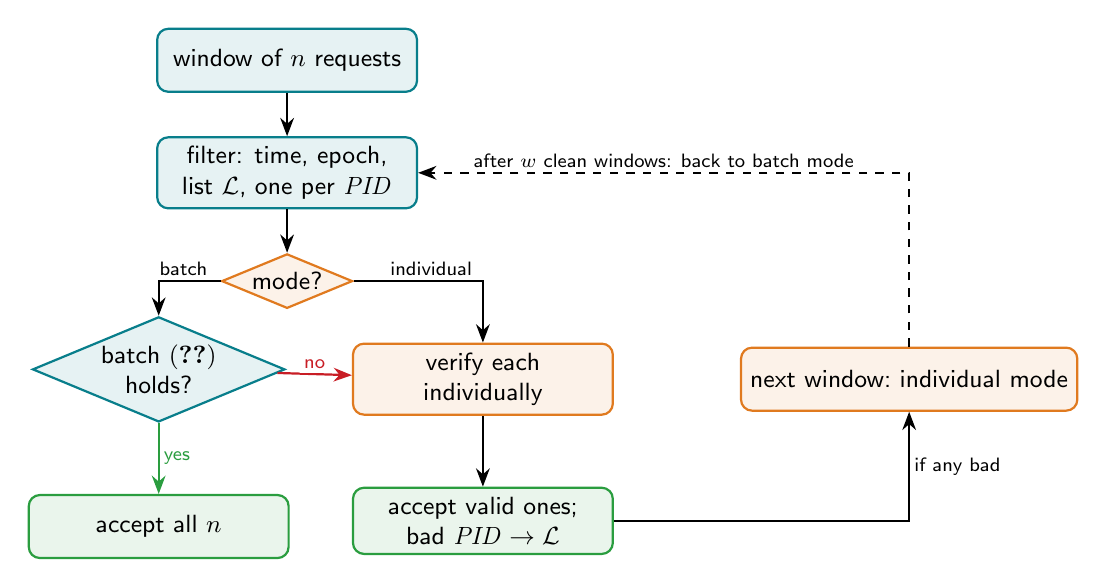
\begin{tikzpicture}[font=\sffamily\small,node distance=0.55cm,
   box/.style={draw=#1,fill=#1!10,rounded corners,thick,minimum width=3.3cm,minimum height=0.8cm,align=center},
   dia/.style={draw=#1,fill=#1!10,diamond,aspect=2.4,thick,align=center,inner sep=1pt}]
  \node[box=uavc] (a) {window of $n$ requests};
  \node[box=uavc,below=of a] (f) {filter: time, epoch,\\ list $\mathcal{L}$, one per $\PID$};
  \node[dia=hoc,below=of f] (m) {mode?};
  \node[dia=uavc,below left=0.6cm and 0.4cm of m] (b) {batch \eqref{eq:bv}\\ holds?};
  \node[box=good,below=0.9cm of b] (ok) {accept all $n$};
  \node[box=hoc,below right=0.6cm and 0.4cm of m] (ind) {verify each\\ individually};
  \node[box=good,below=0.9cm of ind] (acc) {accept valid ones;\\ bad $\PID\to\mathcal{L}$};
  \node[box=hoc,right=1.6cm of ind,minimum width=2.7cm] (sw) {next window:\ individual mode};
  \draw[-{Stealth},thick] (a) -- (f); \draw[-{Stealth},thick] (f) -- (m);
  \draw[-{Stealth},thick] (m) -| node[lbl,pos=0.3,above]{batch} (b);
  \draw[-{Stealth},thick] (m) -| node[lbl,pos=0.3,above]{individual} (ind);
  \draw[-{Stealth},thick,good] (b) -- node[lbl,right]{yes} (ok);
  \draw[-{Stealth},thick,bad] (b) -- node[lbl,above]{no} (ind);
  \draw[-{Stealth},thick] (ind) -- (acc);
  \draw[-{Stealth},thick] (acc.east) -| node[lbl,pos=0.75,right]{if any bad} (sw.south);
  \draw[-{Stealth},thick,dashed] (sw.north) |- node[lbl,pos=0.75,above]{after $w$ clean windows: back to batch mode} (f.east);
\end{tikzpicture}
\caption{Adaptive verification rule of Step UA3.}
\label{fig:fallback}
\end{figure}

\begin{proposition}[Bounded cost under batch poisoning]\label{prop:dos}
For any number $d\ge1$ of invalid requests in a window of $n$, Step UA3 costs at most $T_{BV}(n)+n\,T_{SV}$, and every valid request is accepted. In
individual mode it costs exactly $n\,T_{SV}$. With the constants of~\cite{base}, $n=120$: clean $119.9$\,ms, worst case $448.6$\,ms ($3.7\times$),
individual mode $328.8$\,ms. In the base scheme a single invalid request makes \emph{all} $n$ fail (goodput $0$).
\end{proposition}

\begin{table}[H]
\centering\small
\caption{Verification time at the TUAV for $n=120$ with $d$ invalid requests (average of 200 random placements; \texttt{compute\_results.py}).}
\label{tab:iso}
\resizebox{\linewidth}{!}{%
\pgfplotstabletypeset[
  columns={pct,d,split_ms,fallback_ms,individual_ms,ours_goodput,orig_goodput},
  columns/pct/.style={column name={bad (\%)}},
  columns/d/.style={column name={$d$}},
  columns/split_ms/.style={column name={split-and-retest (ms)},fixed,precision=1},
  columns/fallback_ms/.style={column name={our fallback (ms)},fixed,precision=1},
  columns/individual_ms/.style={column name={individual (ms)},fixed,precision=1},
  columns/ours_goodput/.style={column name={our goodput (\%)}},
  columns/orig_goodput/.style={column name={base goodput (\%)}},
  every head row/.style={before row=\toprule,after row=\midrule},
  every last row/.style={after row=\bottomrule},
  row predicate/.code={\ifnum\pgfplotstablerow>5\relax\ifnum\pgfplotstablerow<10\relax\pgfplotstableuserowfalse\fi\fi}
]\isolation}
\end{table}

\subsection{Rekeying on leave, eviction and join (RK)}
\begin{stepbox}{uavc}{RK1--RK2 \;Group-key update (TUAV)}
\steplabel{uavc}{RK1.} Let $S'$ be the new member set: leavers and evicted members are removed, and joiners are added after their own UA2--UA4. $\Ta$ draws a
\emph{fresh} $\GK'_a$, sets $\nu\leftarrow\nu+1$, and broadcasts $\langle\ID_a,\ts,\nu,\{\Hd(\PID_i),\Enc(K_i,\GK'_a\cat\nu;\,\Hd(\PID_i)\cat\nu\cat\ts)\}_{i\in S'}\rangle$.\\
\steplabel{uavc}{RK2.} Each $\U_i\in S'$ decrypts its entry and switches to $\GK'_a$.
\end{stepbox}
\begin{whybox}
A removed member has no $K_j$ of anyone else, so it cannot open any entry. That is the property the CRT construction lost
(Finding~\ref{f:crt}). A joiner receives only the fresh $\GK'_a$, so it cannot read traffic sent before it joined. A version $\nu$ in the associated
data stops an old ciphertext being replayed as a new key.
\end{whybox}
\paragraph{Optional logarithmic rekeying (LKH).} For very large swarms the TUAV can arrange members as leaves of a binary key tree~\cite{lkh}, using
$K_i$ as leaf keys. A single leave then costs $2\lceil\log_2 n\rceil-1$ ciphertexts (13 for $n=120$) instead of $n-1$. Section~\ref{sec:perf}
reports both variants.

% =====================================================================
\section{C2: The Vehicle Tier}\label{sec:c2}
% =====================================================================
The base paper secures only the UAV--TUAV link and states that vehicle authentication is ``well studied'' and assumed to be handled elsewhere. Yet
the vehicles are why the network exists. Existing vehicle schemes assume an RSU or an online TA, neither of which is available here. C2 brings
vehicles under the \emph{same} offline trust root.

\begin{keybox}
Vehicles carry the same certificateless credential as UAVs. Authenticated UAVs act as \emph{relays and filters}: they carry vehicles' requests to the
TUAV, which batch-verifies them and returns a regional key for V2V traffic. The UAVs cannot read or forge anything.
\end{keybox}

\begin{figure}[H]
\centering
\resizebox{\linewidth}{!}{%
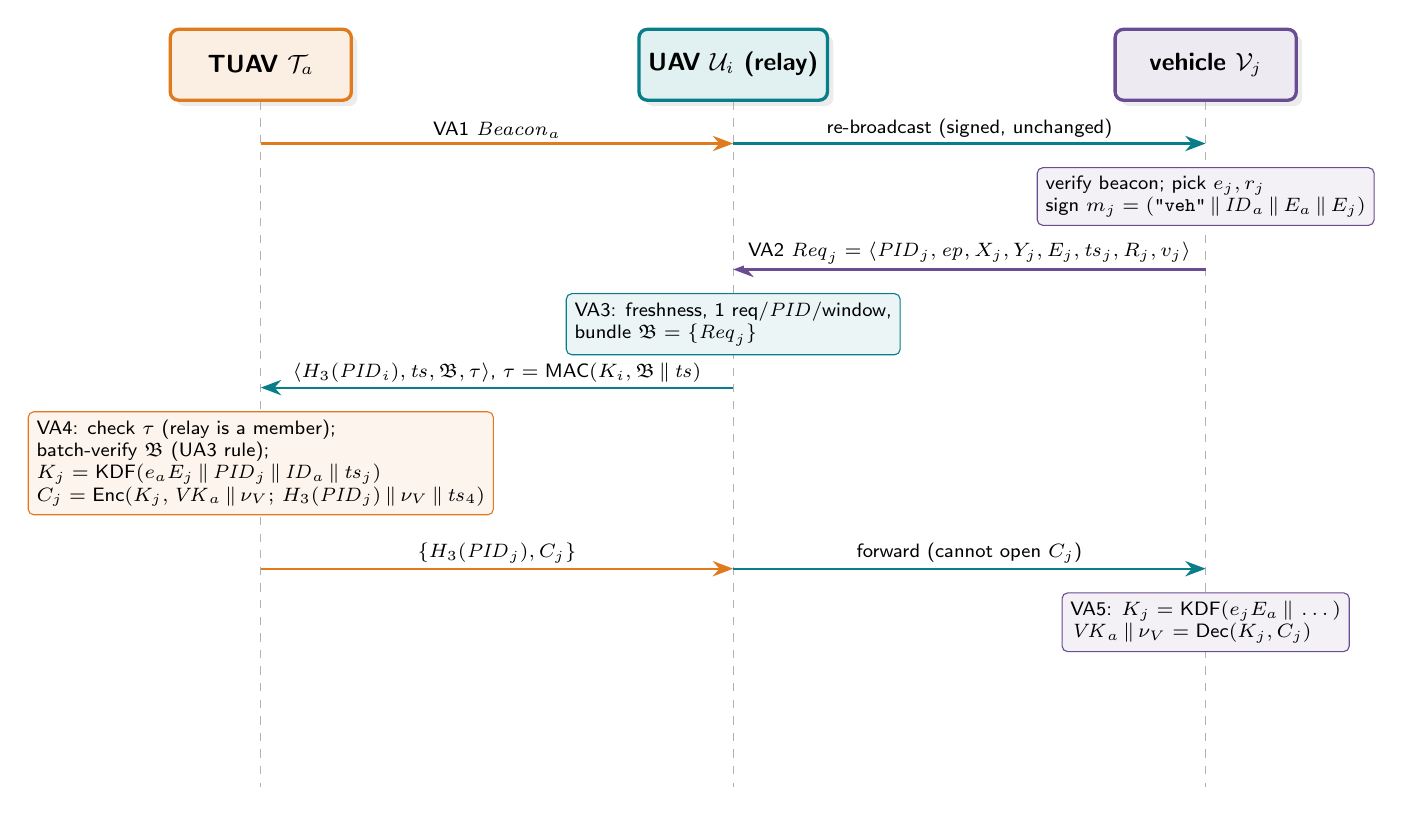
\begin{tikzpicture}[font=\sffamily\small]
  \node[ent=hoc]  (t) at (0,0)   {TUAV $\Ta$};
  \node[ent=uavc] (u) at (6,0)   {UAV $\U_i$ (relay)};
  \node[ent=vehc] (v) at (12,0)  {vehicle $\V_j$};
  \foreach \n in {t,u,v}{ \draw[life] (\n.south) -- ++(0,-8.7); }
  \draw[msg=hoc] (0,-1.0) -- node[lbl,above]{VA1 $\mathit{Beacon}_a$} (6,-1.0);
  \draw[msg=uavc] (6,-1.0) -- node[lbl,above]{re-broadcast (signed, unchanged)} (12,-1.0);
  \node[act=vehc,anchor=north] at (12,-1.3) {verify beacon; pick $e_j,r_j$\\ sign $m_j=(\texttt{"veh"}\cat\ID_a\cat E_a\cat E_j)$};
  \draw[msg=vehc] (12,-2.6) -- node[lbl,above]{VA2 $\mathit{Req}_j=\langle\PID_j,\ep,X_j,Y_j,E_j,\ts_j,R_j,v_j\rangle$} (6,-2.6);
  \node[act=uavc,anchor=north] at (6,-2.9) {VA3: freshness, 1 req/$\PID$/window,\\ bundle $\mathfrak{B}=\{\mathit{Req}_j\}$};
  \draw[msg=uavc] (6,-4.1) -- node[lbl,above]{$\langle\Hd(\PID_i),\ts,\mathfrak{B},\tau\rangle$, $\tau=\MAC(K_i,\mathfrak{B}\cat\ts)$} (0,-4.1);
  \node[act=hoc,anchor=north] at (0,-4.4) {VA4: check $\tau$ (relay is a member);\\ batch-verify $\mathfrak{B}$ (UA3 rule);\\ $K_j=\KDF(e_aE_j\cat\PID_j\cat\ID_a\cat\ts_j)$\\ $C_j=\Enc(K_j,\VK_a\cat\nu_V;\,\Hd(\PID_j)\cat\nu_V\cat\ts_4)$};
  \draw[msg=hoc] (0,-6.4) -- node[lbl,above]{$\{\Hd(\PID_j),C_j\}$} (6,-6.4);
  \draw[msg=uavc] (6,-6.4) -- node[lbl,above]{forward (cannot open $C_j$)} (12,-6.4);
  \node[act=vehc,anchor=north] at (12,-6.7) {VA5: $K_j=\KDF(e_jE_a\cat\dots)$\\ $\VK_a\cat\nu_V=\Dec(K_j,C_j)$};
\end{tikzpicture}}
\caption{C2: vehicle authentication relayed by an authenticated UAV.}
\label{fig:c2}
\end{figure}

\subsection{Steps}
\begin{stepbox}{vehc}{VA1--VA5 \;Vehicle admission}
\steplabel{vehc}{VA1.} UAVs re-broadcast the TUAV's signed beacon so that vehicles out of the TUAV's range receive it. A relay cannot alter it.\\[2pt]
\steplabel{vehc}{VA2.} $\V_j$ verifies the beacon, picks $e_j,r_j$, and signs $m_j=(\texttt{"veh"}\cat\ID_a\cat E_a\cat E_j)$ exactly as in UA2, giving
$\mathit{Req}_j$. It sends the request to a UAV in range, or directly to $\Ta$ if it is in range.\\[2pt]
\steplabel{vehc}{VA3.} The relay $\U_i$ checks freshness, allows at most one request per $\PID_j$ per window, collects a bundle $\mathfrak{B}$ and sends
$\langle\Hd(\PID_i),\ts,\mathfrak{B},\tau=\MAC(K_i,\mathfrak{B}\cat\ts)\rangle$ to $\Ta$.\\[2pt]
\steplabel{vehc}{VA4.} $\Ta$ discards the bundle unless $\tau$ verifies under the key of a \emph{current} member. It then applies the UA3 rule to
$\mathfrak{B}$, derives $K_j$ for each valid vehicle, and returns $C_j=\Enc(K_j,\VK_a\cat\nu_V;\,\Hd(\PID_j)\cat\nu_V\cat\ts_4)$ through $\U_i$.\\[2pt]
\steplabel{vehc}{VA5.} $\V_j$ derives $K_j$, decrypts $\VK_a$ and erases $e_j$. A successful decryption authenticates $\Ta$.
\end{stepbox}

\subsection{V2V communication under the regional key}
Vehicles send two classes of message:
\begin{itemize}
  \item \textbf{Routine beacons} (position, speed; about 10 per second):\ $\langle m,\PID_j,\ts,\MAC(\VK_a,m\cat\PID_j\cat\ts)\rangle$. Cost: one HMAC.
  \item \textbf{Safety-critical events} (accident, road blocked): $\langle m,\PID_j,\ep,X_j,Y_j,\ts,R,v\rangle$ with a certificateless signature as in UA2.
        Receivers verify bursts of events with the batch test~\eqref{eq:bv}.
\end{itemize}

\begin{whybox}
\begin{itemize}[leftmargin=*]
  \item \textbf{Same credential, same root.} One registration serves both UAVs and vehicles, so a vehicle can be verified anywhere using only $\Ppub$.
  \item \textbf{UAVs relay, the TUAV verifies.} Battery-limited UAVs do no public-key verification for vehicles. The TUAV, which has a cable power supply, does the batch work, where batching pays off most (hundreds of vehicles).
  \item \textbf{Relay MAC as a flood filter.} Only bundles from current members reach the verifier, and each relay rate-limits per pseudonym. An outsider flooding forged requests is
        stopped at the first hop, which addresses the denial-of-service gap of Finding~\ref{f:proof}(iv) at the vehicle scale.
  \item \textbf{Separate keys $\VK_a$ and $\GK_a$.} A captured vehicle must not obtain the UAV control-channel key (privilege separation).
  \item \textbf{Two message classes.} A MAC under a shared key is fast but only proves ``some member sent this''. Safety-critical events need
        non-repudiation (accountability after an accident), so they are signed.
\end{itemize}
\end{whybox}
\begin{limitbox}
Any holder of $\VK_a$ can forge a \emph{routine} beacon that appears to come from another pseudonym. We accept this for routine traffic and require signatures
for events that matter. A relay UAV can drop bundles (denial of service) but cannot forge, read or alter them undetected.
\end{limitbox}

% =====================================================================
\section{C3: TUAV-to-TUAV Handover}\label{sec:c3}
% =====================================================================
One TUAV covers a limited area, so a real disaster zone needs several, and UAVs and vehicles move between cells. Re-running the full C1/C2
admission at every cell border costs signature generation and verification on both sides and interrupts service. The base paper considers a single TUAV only.

\begin{keybox}
Neighbouring TUAVs share a link key $K_{ab}$. The old TUAV gives a moving member an encrypted \emph{ticket}. The new TUAV opens the ticket,
checks a MAC, runs one ECDH for forward secrecy, and admits the member \emph{without any signature verification and without the TA}.
\end{keybox}

\begin{figure}[H]
\centering
\resizebox{\linewidth}{!}{%
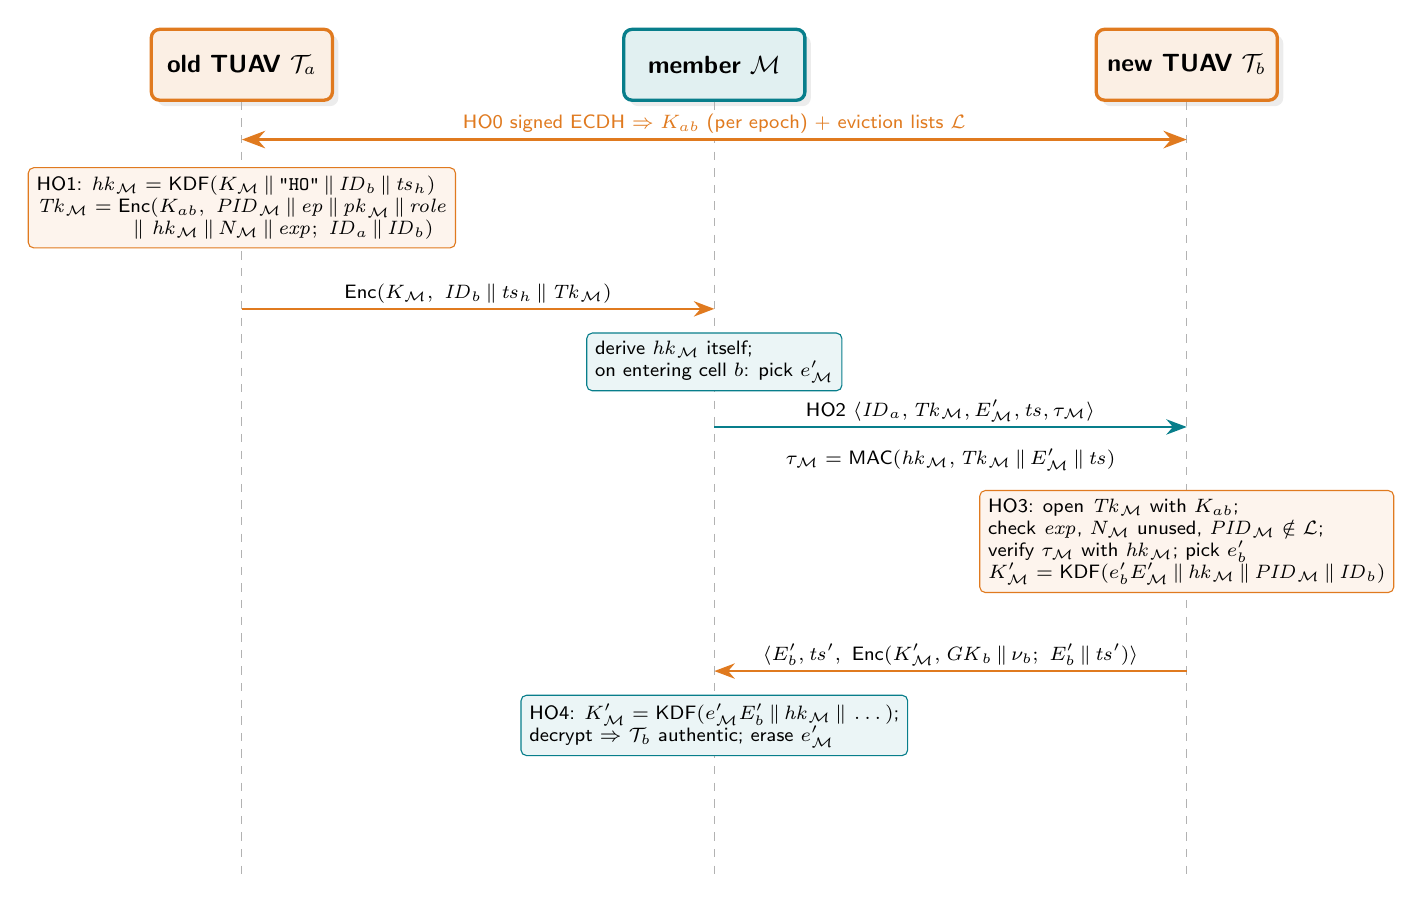
\begin{tikzpicture}[font=\sffamily\small]
  \node[ent=hoc] (a) at (0,0)  {old TUAV $\Ta$};
  \node[ent=uavc] (m) at (6,0) {member $\M$};
  \node[ent=hoc] (b) at (12,0) {new TUAV $\Tb$};
  \foreach \n in {a,m,b}{ \draw[life] (\n.south) -- ++(0,-9.9); }
  \draw[{Stealth}-{Stealth},hoc,very thick] (0,-0.95) -- node[lbl,above]{HO0 signed ECDH $\Rightarrow K_{ab}$ (per epoch) + eviction lists $\mathcal{L}$} (12,-0.95);
  \node[act=hoc,anchor=north] at (0,-1.3) {HO1: $\hk_\M=\KDF(K_\M\cat\texttt{"HO"}\cat\ID_b\cat\ts_h)$\\ $\Tk_\M=\Enc(K_{ab},\ \PID_\M\cat\ep\cat\pk_\M\cat\mathit{role}$\\ \hspace*{4.5em}$\cat\,\hk_\M\cat N_\M\cat\mathit{exp};\ \ID_a\cat\ID_b)$};
  \draw[msg=hoc] (0,-3.1) -- node[lbl,above]{$\Enc(K_\M,\ \ID_b\cat\ts_h\cat\Tk_\M)$} (6,-3.1);
  \node[act=uavc,anchor=north] at (6,-3.4) {derive $\hk_\M$ itself;\\ on entering cell $b$: pick $e'_\M$};
  \draw[msg=uavc] (6,-4.6) -- node[lbl,above]{HO2 $\langle\ID_a,\Tk_\M,E'_\M,\ts,\tau_\M\rangle$} (12,-4.6);
  \node[font=\scriptsize\sffamily,anchor=north] at (9,-4.75) {$\tau_\M=\MAC(\hk_\M,\Tk_\M\cat E'_\M\cat\ts)$};
  \node[act=hoc,anchor=north] at (12,-5.4) {HO3: open $\Tk_\M$ with $K_{ab}$;\\ check $\mathit{exp}$, $N_\M$ unused, $\PID_\M\notin\mathcal{L}$;\\ verify $\tau_\M$ with $\hk_\M$; pick $e'_b$\\ $K'_\M=\KDF(e'_bE'_\M\cat\hk_\M\cat\PID_\M\cat\ID_b)$};
  \draw[msg=hoc] (12,-7.7) -- node[lbl,above]{$\langle E'_b,\ts',\ \Enc(K'_\M,\GK_b\cat\nu_b;\ E'_b\cat\ts')\rangle$} (6,-7.7);
  \node[act=uavc,anchor=north] at (6,-8.0) {HO4: $K'_\M=\KDF(e'_\M E'_b\cat\hk_\M\cat\dots)$;\\ decrypt $\Rightarrow$ $\Tb$ authentic; erase $e'_\M$};
\end{tikzpicture}}
\caption{C3 handover. Only symmetric operations and one ECDH are needed at the new TUAV.}
\label{fig:c3}
\end{figure}

\subsection{Steps}
\begin{stepbox}{hoc}{HO0--HO4 \;Inter-TUAV link and ticket-based handover}
\steplabel{hoc}{HO0.} When two TUAVs come into range, and once per epoch after that, they exchange signed ephemeral values $(E_{ab},E_{ba})$ using their
credentials and derive $K_{ab}=\KDF(e_{ab}E_{ba}\cat\ID_a\cat\ID_b\cat\ts)$. Over $K_{ab}$ they exchange their eviction lists $\mathcal{L}$.\\[2pt]
\steplabel{hoc}{HO1.} When member $\M$ (pairwise key $K_\M$ with $\Ta$) approaches cell $b$, $\Ta$ derives $\hk_\M=\KDF(K_\M\cat\texttt{"HO"}\cat\ID_b\cat\ts_h)$,
draws a nonce $N_\M$ and an expiry $\mathit{exp}$, builds the ticket
$\Tk_\M=\Enc(K_{ab},\ \PID_\M\cat\ep\cat\pk_\M\cat\mathit{role}\cat\hk_\M\cat N_\M\cat\mathit{exp};\ \ID_a\cat\ID_b)$, and sends it to $\M$ under $K_\M$.
$\M$ derives the same $\hk_\M$ from $K_\M$.\\[2pt]
\steplabel{hoc}{HO2.} In cell $b$, $\M$ picks $e'_\M$ and sends $\langle\ID_a,\Tk_\M,E'_\M,\ts,\tau_\M=\MAC(\hk_\M,\Tk_\M\cat E'_\M\cat\ts)\rangle$ to $\Tb$.\\[2pt]
\steplabel{hoc}{HO3.} $\Tb$ decrypts $\Tk_\M$ with $K_{ab}$ and rejects the request if $\mathit{exp}$ has passed, if $N_\M$ was already used (it caches nonces until
$\mathit{exp}$), if $\Hd(\PID_\M)\in\mathcal{L}$, or if $\tau_\M$ does not verify under $\hk_\M$. Otherwise it picks $e'_b$ and sends
$\langle E'_b,\ts',\Enc(K'_\M,\GK_b\cat\nu_b;\,E'_b\cat\ts')\rangle$ with $K'_\M=\KDF(e'_bE'_\M\cat\hk_\M\cat\PID_\M\cat\ID_b)$. For a vehicle
($\mathit{role}=\texttt{veh}$), it sends $\VK_b$ instead of $\GK_b$.\\[2pt]
\steplabel{hoc}{HO4.} $\M$ derives $K'_\M$ and decrypts. Success means $\Tb$ knows $\hk_\M$, which only a holder of $K_{ab}$ could obtain, so $\Tb$ is authentic.
$\M$ and $\Tb$ erase $e'_\M,e'_b$. $\Ta$ removes $\M$ at its next rekey.
\end{stepbox}

\begin{whybox}
\begin{itemize}[leftmargin=*]
  \item \textbf{Why a ticket.} The old TUAV already verified $\M$'s signature. The ticket passes that verified fact on, under $K_{ab}$, so the new TUAV need not repeat the work.
  \item \textbf{Why $\hk_\M$ and not $K_\M$.} $\Tb$ never learns the pairwise key $\M$ used in cell $a$. If $\Tb$ is later compromised, $\M$'s traffic in cell $a$ stays safe.
  \item \textbf{Why a fresh ECDH.} The new key $K'_\M$ mixes a fresh Diffie--Hellman value with $\hk_\M$, so it has forward secrecy, and an attacker who later
        learns $K_{ab}$ still cannot compute it.
  \item \textbf{Why nonce, expiry and AD.} A ticket can be used once, only before $\mathit{exp}$, and only between the two named TUAVs ($\ID_a\cat\ID_b$ as associated data).
  \item \textbf{Why share $\mathcal{L}$.} An entity evicted in cell $a$ cannot escape by moving to cell $b$.
\end{itemize}
\end{whybox}

% =====================================================================
\section{The TA's Offline Role: Tracing and Global Revocation}\label{sec:tr}
% =====================================================================
\begin{stepbox}{deep}{TR1--TR2 \;(TA, whenever reachable -- never on the critical path)}
\steplabel{deep}{TR1 (tracing).} Given a pseudonym from a disputed message, the tracing office computes
$\RID=\PID^2\oplus\Hz(t\cdot\PID^1\cat\ep)$, which is correct because $t\,\PID^1=t\rho P=\rho\Tpub$. The signed message and the RG1 record bind the real
entity to the act (non-repudiation).\\[2pt]
\steplabel{deep}{TR2 (global revocation).} To ban an entity permanently, $\TA$ publishes a signed list of $\Hd(\PID^{(\ep)})$ for all of its \emph{remaining}
epochs. TUAVs merge the list into $\mathcal{L}$ and propagate it over $K_{ab}$. Earlier pseudonyms are not published, so the entity's past stays unlinkable.
\end{stepbox}
\begin{whybox}
Revocation becomes \emph{two-speed}. A TUAV evicts a misbehaving pseudonym \emph{immediately and locally} (UA3, RK1, shared via HO0), which covers the
rest of the epoch. Permanent revocation waits until the TA is reachable, by any channel at any time, and it never blocks authentication. This is the
practical meaning of ``infrastructure-less'': the infrastructure \emph{helps when present} but is \emph{not required}.
\end{whybox}

% =====================================================================
\section{Security Analysis}\label{sec:security}
% =====================================================================
We give proof \emph{sketches} that follow standard techniques; the full game-based proofs and a mechanised ProVerif~\cite{proverif} analysis are part of the
final report (Section~\ref{sec:plan}). Unlike the base paper's Theorem~1 (Finding~\ref{f:proof}), every reduction below embeds the challenge in a value that
is \emph{secret}.

\subsection{Authority independence}
\begin{proposition}[No online TA]\label{prop:indep}
Steps UA1--UA5, RK1--RK2, VA1--VA5 and HO0--HO4 use only (a) the public $\mathit{params}$, including $\Ppub$, (b) keys stored by the participating
entities, and (c) messages exchanged between them. No step sends a message to, or waits for a message from, the TA.
\end{proposition}
\begin{proof}
By inspection of each step. Signature verification needs $\Ppub$ only (equation~\eqref{eq:bv}); key derivation uses ephemeral values and stored pairwise keys; tickets use $K_{ab}$.
\end{proof}
\noindent Consequently the success probability of authentication is independent of the TA-link availability $A$ (Figure~\ref{fig:avail}), whereas for the base scheme it equals $A$.

\subsection{Unforgeability, escrow-freeness and non-repudiation}
\begin{theorem}[EUF-CMA]\label{thm:euf}
In the random-oracle model, if ECDLP is hard in $\G$, no PPT Type-I or Type-II adversary can produce a valid signature $(R,v)$ on a new message under the
public key of an honest entity, except with negligible probability.
\end{theorem}
\begin{proof}[Proof sketch]
\emph{Type II (malicious TA, knows $s$ and every $d$).} The reduction $\mathcal{B}$ receives $A=aP$, guesses the target entity, and sets its
$X^*=A$; it knows $s$ and can produce all partial keys. It answers signing queries for the target without $x^*$ by programming the oracle: it picks
$v,c$ at random, sets $R=vP-c\,\pk^*$ and defines $\Ht(\cdot)=c$. From a forgery, the forking lemma~\cite{forking} gives two signatures with the same $R$ and
different challenges $c\ne c'$. Then $\sk^*=(v-v')/(c-c')$ and $a=x^*=\sk^*-d^*$.\\
\emph{Type I (outsider, may replace public keys).} $\mathcal{B}$ sets $\Ppub=A$. It issues partial keys without $s$ by choosing $d,h$ at random and setting
$Y=dP-h\Ppub$ and $\Ho(\PID,\ep,X,Y)=h$. A forgery under a (possibly replaced) key $\pk^*=X^*+Y^*+h^*\Ppub$ is forked on $\Ht$, which gives
$\sk^*=\log_P(X^*+Y^*)+h^*a$. Forking again at the $\Ho$ query that fixed $h^*$ gives $\sk^{*\prime}$ with $h^{*\prime}\ne h^*$ and the same $X^*+Y^*$, hence
$a=(\sk^*-\sk^{*\prime})/(h^*-h^{*\prime})$. This is the standard double-forking argument for pairing-free certificateless and identity-based Schnorr signatures.
\end{proof}

\begin{theorem}[Escrow-freeness and non-repudiation]\label{thm:escrow}
The TA cannot produce a signature that verifies under a registered entity's public key, so a valid signature (or a valid UA2 request) can be attributed to that entity.
\end{theorem}
\begin{proof}
This is the Type-II case of Theorem~\ref{thm:euf}. The TA's knowledge ($s$, $d_\Ent$, $\PID_\Ent$) does not include $x_\Ent$, and the RG1 proof of possession binds
$X_\Ent$ to $\RID_\Ent$. (Contrast with Finding~\ref{f:escrow}.)
\end{proof}

\subsection{Batch soundness}
\begin{theorem}[Small-exponent test~\cite{bgr}]\label{thm:batch}
If at least one request in a batch is invalid, equation~\eqref{eq:bv} holds with probability at most $2^{-\ell_\lambda}$ over the choice of the weights $\lambda_i$.
\end{theorem}
\begin{proof}[Proof sketch]
Write $\Delta_i=v_iP-R_i-c_i\pk_i$, with $\Delta_k\ne O$ for some $k$. Equation~\eqref{eq:bv} is $\sum_i\lambda_i\Delta_i=O$. Fix all $\lambda_i$ with $i\ne k$. Because $\G$
has prime order, at most one value of $\lambda_k$ satisfies the equation, so the probability is at most $2^{-\ell_\lambda}$. The cancellation attack of
Finding~\ref{f:proof}(iii) is therefore defeated.
\end{proof}

\subsection{Mutual authentication and key secrecy}
\begin{theorem}[C1 key secrecy and mutual authentication]\label{thm:key}
Under CDH in the random-oracle model and the security of the AEAD scheme: (i) only $\Ta$ and $\U_i$ can compute $K_i$; (ii) $\GK_a$ is known only to $\Ta$ and the
current members; (iii) $\Ta$ accepts $\U_i$ only if $\U_i$ signed $E_i$ for this beacon; (iv) $\U_i$ accepts only the TUAV that signed $E_a$.
\end{theorem}
\begin{proof}[Proof sketch]
(i) $K_i=\KDF(e_ae_iP\cat\dots)$. An adversary sees $E_a,E_i$ only, and computing $e_ae_iP$ is CDH. Swapping $E_i$ would break the signature on $m_i$
(Theorem~\ref{thm:euf}), and swapping $E_a$ would break the beacon signature.
(ii) $C_i$ is AEAD under $K_i$. An insider $\U_k$ knows only its own $K_k$, which is independent of every other $K_i$ (unlike Lemma~\ref{lem:leak}).
(iii) The request signature covers $E_a,\ID_a,E_i,\ts_i$.
(iv) Decryption of $C_i$ under $K_i$ succeeds only if the sender knows $e_a$, and $E_a$ is signed by $\sk_a$.
\end{proof}

\begin{theorem}[Forward secrecy, and key secrecy under membership change]\label{thm:fs}
(a) Compromise of every long-term key ($x,d$ of members, $\sk_a$ of the TUAV, even $s$ and $t$) after a session does not reveal that session's $K_i$ or $\GK_a$.
(b) A member removed in RK1 cannot obtain $\GK'_a$ (group forward secrecy). (c) A member that joins cannot obtain an earlier $\GK_a$ (group backward secrecy).
\end{theorem}
\begin{proof}[Proof sketch]
(a) $K_i$ depends on the erased $e_a,e_i$; long-term keys only authenticate. (b) $\GK'_a$ is fresh and encrypted only under $\{K_i\}_{i\in S'}$; the removed
member knows none of them. This is the property the base scheme loses by Lemma~\ref{lem:leak}. (c) The joiner receives only the fresh $\GK'_a$.
\end{proof}

\subsection{Privacy}
\begin{theorem}[Anonymity, epoch-unlinkability, traceability]\label{thm:priv}
(i) An eavesdropper, or any entity other than the holder of $t$, learns nothing about $\RID_\Ent$ from $\PID_\Ent$. (ii) Requests from different epochs cannot be linked.
(iii) The holder of $t$ can recover $\RID_\Ent$ from any $\PID_\Ent$.
\end{theorem}
\begin{proof}[Proof sketch]
(i) $\PID^2=\RID\oplus\Hz(\rho\Tpub\cat\ep)$ is hashed-ElGamal encryption; computing $\rho\Tpub$ from $\PID^1=\rho P$ and $\Tpub=tP$ is CDH. (ii) All
values that appear in a request ($\PID^1,\PID^2,X,Y,E,R,v$) are freshly random per epoch, because RG uses independent $\rho,y,x^{(\ep)}$. (iii) TR1.
\end{proof}
\begin{limitbox}
Within \emph{one} epoch an entity uses one pseudonym, so its sessions in that epoch are linkable. This is a deliberate trade-off: it makes local
eviction effective (an evicted pseudonym cannot be replaced until the next epoch). The epoch length sets the balance; the base paper's per-session pseudonyms
resolvable only by the TA cannot support local eviction at all.
\end{limitbox}

\subsection{Replay and handover security}
\begin{theorem}[Replay resistance]\label{thm:replay}
A recorded request, ACK, bundle or handover message is rejected outside its session.
\end{theorem}
\begin{proof}[Proof sketch]
Requests sign $(\ID_a,E_a,\ts_i)$, and $E_a$ changes every beacon period. ACK and rekey entries carry $\nu$ and $\ts$ in their associated data. Bundles carry $\ts$ under
$\tau$. Tickets carry a single-use nonce $N_\M$ cached until $\mathit{exp}$, and $\tau_\M$ binds the fresh $E'_\M$ and $\ts$.
\end{proof}
\begin{theorem}[Handover]\label{thm:ho}
(i) Only $\Ta,\Tb$ can open or create a valid ticket. (ii) Only the member that holds $K_\M$ can use its ticket. (iii) $K'_\M$ is secret even against a later compromise
of $K_{ab}$, $K_\M$ or long-term keys. (iv) $\Tb$ never learns $K_\M$.
\end{theorem}
\begin{proof}[Proof sketch]
(i) AEAD under $K_{ab}$ with $\ID_a\cat\ID_b$ as associated data. (ii) $\tau_\M$ requires $\hk_\M=\KDF(K_\M\cat\dots)$. (iii) $K'_\M$ mixes $e'_be'_\M P$ (CDH, ephemeral).
(iv) The ticket contains $\hk_\M$, a one-way derivative of $K_\M$.
\end{proof}

\subsection{Security comparison}
\begin{table}[H]
\centering\small
\caption{Security properties. \yes\ holds, \no\ fails, \halfmark\ partially. ``Base (claimed)'' is Table~II of~\cite{base}; ``Base (actual)'' is our analysis.}
\label{tab:seccomp}
\resizebox{\linewidth}{!}{%
\begin{tabular}{@{}llccc@{}}
\toprule
& Property & Base (claimed) & Base (actual) & \textbf{Ours}\\
\midrule
F1 & Unforgeability (with valid proof) & \yes & \halfmark\ proof empty (F.\,5) & \yes\ Thm \ref{thm:euf}\\
F2 & Conditional privacy & \yes & \yes & \yes\ Thm \ref{thm:priv}\\
F3 & Session/group key establishment & \yes & \halfmark\ leaks to members (F.\,4) & \yes\ Thm \ref{thm:key}\\
F4 & Key-escrow resilience & \yes & \no\ (F.\,2) & \yes\ Thm \ref{thm:escrow}\\
F5 & Scalability & \yes & \no\ $O(n^3)$ bytes (F.\,4) & \yes\ $68n$ B\\
F6 & Dynamic identity updating & \yes & \yes & \yes\ per epoch\\
F7 & Forward secrecy & \yes & \no\ (F.\,3) & \yes\ Thm \ref{thm:fs}\\
F8 & Batch validation (sound) & \yes & \halfmark\ no weights, no fallback & \yes\ Thm \ref{thm:batch}, Prop.\,\ref{prop:dos}\\
F9 & Unlinkability & \yes & \yes\ per session & \halfmark\ per epoch\\
F10 & Non-repudiation & \yes & \no\ (F.\,2) & \yes\ Thm \ref{thm:escrow}\\
F11 & Replay resistance & \yes & \yes & \yes\ Thm \ref{thm:replay}\\
\midrule
N1 & Works without online TA & -- & \no\ (F.\,1) & \yes\ Prop.\,\ref{prop:indep}\\
N2 & Secure revocation (leavers locked out) & -- & \no\ (F.\,4) & \yes\ Thm \ref{thm:fs}\\
N3 & Bounded cost under batch poisoning & -- & \no & \yes\ Prop.\,\ref{prop:dos}\\
N4 & Vehicle tier & -- & \no\ out of scope & \yes\ C2\\
N5 & Multi-TUAV handover & -- & \no & \yes\ Thm \ref{thm:ho}\\
\bottomrule
\end{tabular}}
\end{table}

% =====================================================================
\section{Performance Analysis}\label{sec:perf}
% =====================================================================
\paragraph{Method.} For a fair comparison we use \emph{exactly} the operation timings of the base paper (MIRACL, 80-bit level, Section~VI-A of~\cite{base}):
$T_P=7.2232$, $T_{SM\text{-}P}=2.6784$, $T_{PA\text{-}P}=0.0342$, $T_{SM\text{-}E}=0.9018$, $T_{SSM\text{-}E}=0.0475$, $T_{PA\text{-}E}=0.0107$,
$T_{ME}=0.6256$, $T_{SH}=0.0012$\,ms. Symmetric operations (KDF, AEAD, MAC on short inputs) are charged as $T_{SH}$. Sizes also follow the base paper:
$|\G|=40$\,B, $|\G_1|=|\G_2|=128$\,B, hash 20\,B, timestamp 4\,B; an AEAD ciphertext of a 16-byte key with version, nonce and tag is 48\,B. All numbers are produced by
\texttt{scripts/compute\_results.py}.
\begin{limitbox}
These are \emph{analytical} costs (operation counts times published timings), the same method the base paper used. Real measurements on a prototype are
planned (Section~\ref{sec:plan}). Both schemes are priced with the same constants, so the comparison is fair even though absolute values on real hardware will differ.
\end{limitbox}

\subsection{Computation}
\begin{table}[H]
\centering\small
\caption{Computation cost (ms). ``Base (honest)'' adds the TA's GA2 work ($29.7414$\,ms per UAV) and places $\Gamma_i$ in $\G_1$.}
\label{tab:comp}
\begin{tabularx}{\linewidth}{@{}>{\raggedright\arraybackslash}X ccc@{}}
\toprule
Operation & Base (reported) & Base (honest) & \textbf{Ours}\\
\midrule
UAV signing & $1.8203$ & $5.3970$ & $\mathbf{1.8048}$ \;($2T_{SM\text{-}E}+T_{SH}$)\\
Single verification & $2.1578$ & $31.8992$ + RTT & $\mathbf{2.7399}$ \;($3T_{SM\text{-}E}+3T_{PA\text{-}E}+2T_{SH}$)\\
Group verification, $n$ & $1.2524n+0.9054$ & $30.9938n+0.9054$ + RTT & $\mathbf{0.9838n+1.8036}$\\
\quad at $n=120$ & $151.19$ & $3720.16$ + RTT & $\mathbf{119.86}$\\
Group verification + key delivery, $n=120$ & not reported & $\ge 3720.16$ + RTT & $\mathbf{228.36}$ \;($1.8880n+1.8036$)\\
Member: receive key (incl.\ beacon check) & not reported & -- & $3.6441$\\
\bottomrule
\end{tabularx}
\end{table}

\begin{figure}[H]
\centering
\begin{tikzpicture}
\begin{axis}[width=0.92\linewidth,height=7.4cm,xlabel={number of UAVs $n$},ylabel={TUAV-side cost (ms)},
   xmin=20,xmax=120,ymin=0,ymax=4000,legend style={at={(0.5,-0.18)},anchor=north,legend columns=3},
   cycle list={{bad,very thick,mark=*},{bad,dashed,mark=o},{black!45,mark=square},{black!45,mark=triangle},{black!45,mark=diamond},{black!45,mark=x},{uavc,very thick,mark=*},{good,very thick,mark=square*}}]
  \addplot table[x=n,y=orig_honest]{\gacost}; \addlegendentry{Base, honest (TA pairings incl.)}
  \addplot table[x=n,y=orig]{\gacost};        \addlegendentry{Base, as reported}
  \addplot table[x=n,y=kumar]{\gacost};       \addlegendentry{Kumar et al.}
  \addplot table[x=n,y=xu]{\gacost};          \addlegendentry{Xu et al.}
  \addplot table[x=n,y=mei]{\gacost};         \addlegendentry{Mei et al.}
  \addplot table[x=n,y=ali]{\gacost};         \addlegendentry{Ali et al.}
  \addplot table[x=n,y=ours_bv]{\gacost};     \addlegendentry{\textbf{Ours: batch verification}}
  \addplot table[x=n,y=ours_total]{\gacost};  \addlegendentry{\textbf{Ours: verification + key delivery}}
\end{axis}
\end{tikzpicture}
\caption{Group authentication cost versus $n$ (satellite RTT \emph{not} added to the base scheme here). Counted honestly, the base scheme is the most expensive of all six.}
\label{fig:gacost}
\end{figure}

\begin{figure}[H]
\centering
\begin{tikzpicture}
\begin{axis}[width=0.48\linewidth,height=6.2cm,xlabel={number of UAVs $n$},ylabel={time to authenticate + key (ms)},
   xmin=20,xmax=120,ymin=0,ymax=6000,legend pos=north west,legend style={font=\tiny\sffamily}]
  \addplot[bad,very thick,mark=*] table[x=n,y=orig_geo]{\etoe}; \addlegendentry{Base, GEO (RTT 600)}
  \addplot[hoc,very thick,mark=triangle*] table[x=n,y=orig_leo]{\etoe}; \addlegendentry{Base, LEO (RTT 50)}
  \addplot[bad,dashed,mark=o] table[x=n,y=orig_reported]{\etoe}; \addlegendentry{Base, as reported}
  \addplot[uavc,very thick,mark=square*] table[x=n,y=ours]{\etoe}; \addlegendentry{Ours (no link)}
\end{axis}
\end{tikzpicture}\hfill
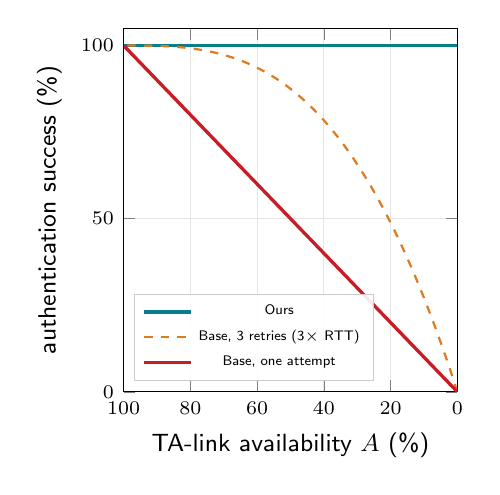
\begin{tikzpicture}
\begin{axis}[width=0.48\linewidth,height=6.2cm,xlabel={TA-link availability $A$ (\%)},ylabel={authentication success (\%)},
   xmin=0,xmax=100,ymin=0,ymax=105,legend pos=south west,legend style={font=\tiny\sffamily},x dir=reverse]
  \addplot[uavc,very thick,domain=0:100,samples=2] {100}; \addlegendentry{Ours}
  \addplot[hoc,thick,dashed,domain=0:100,samples=60] {100*(1-(1-x/100)^3)}; \addlegendentry{Base, 3 retries (3$\times$ RTT)}
  \addplot[bad,very thick,domain=0:100,samples=2] {x}; \addlegendentry{Base, one attempt}
\end{axis}
\end{tikzpicture}
\caption{Left: end-to-end time with the satellite round trip charged to the base scheme. Right: \emph{analytical} availability. The base scheme falls to
zero with the link; ours does not depend on it (Proposition~\ref{prop:indep}).}
\label{fig:avail}
\end{figure}

\begin{whybox}[title={Why our scheme is faster even though the TUAV now verifies}]
The base scheme looks cheap only because the expensive part (three pairings per UAV, about 21.7\,ms) runs on the TA and is left out of the count. Our
verification needs no pairings at all: a batch costs about one elliptic-curve scalar multiplication (0.90\,ms) per UAV. Removing the TA from the loop therefore
\emph{reduces} the total work while also removing the wide-area round trip. The extra cost we \emph{do} add is the per-member ECDH for key delivery ($0.90$\,ms per
UAV), which buys forward secrecy and secure revocation.
\end{whybox}

\subsection{Communication}
\begin{table}[H]
\centering\small
\caption{Communication overhead (bytes).}
\label{tab:comm}
\begin{tabularx}{\linewidth}{@{}>{\raggedright\arraybackslash}X ccc@{}}
\toprule
Message & Base (reported) & Base (honest) & \textbf{Ours}\\
\midrule
Join request (per UAV) & 104 & 192 ($\Gamma_i\in\G_1$) & 248\\
Satellite traffic (per UAV) & -- & 192 up + 512 down & \textbf{0}\\
Key delivery, $n=120$ (all members) & -- & 16.72 MiB & \textbf{8.0 KiB} ($68n+4$)\\
TUAV beacon (per period) & -- & 172 ($Q_{tu}\in\G_1$) & 204\\
Rekey after one leave, $n=120$ & -- & 16.3 MiB & 7.9 KiB (flat) \;/\; \textbf{680 B} (LKH)\\
\bottomrule
\end{tabularx}
\end{table}

\begin{figure}[H]
\centering
\begin{tikzpicture}
\begin{axis}[width=0.92\linewidth,height=6.6cm,ymode=log,xlabel={number of UAVs $n$},ylabel={bytes for group-key delivery (log scale)},
   xmin=10,xmax=120,ymax=1e9,legend style={at={(0.5,-0.22)},anchor=north,legend columns=2},log basis y=10]
  \addplot[bad,very thick,mark=*] table[x=n,y=crt_total]{\keybytes}; \addlegendentry{Base: CRT coefficients to each of $n$ UAVs (measured)}
  \addplot[bad,dashed,mark=o] table[x=n,y=crt_per_ack]{\keybytes}; \addlegendentry{Base: one ACK}
  \addplot[black!45,mark=triangle] table[x=n,y=paper_claim]{\keybytes}; \addlegendentry{Base paper's Table V ($104n$)}
  \addplot[uavc,very thick,mark=square*] table[x=n,y=ours_total]{\keybytes}; \addlegendentry{Ours: one ACK with $n$ entries ($68n+4$)}
\end{axis}
\end{tikzpicture}
\caption{Group-key delivery traffic. The base scheme grows as $O(n^3)$ bytes; ours grows linearly, and at $n=120$ is about 2150$\times$ smaller.}
\label{fig:keybytes}
\end{figure}

\begin{whybox}[title={The trade-off we accept}]
Our join request is larger (248\,B against 192\,B honest or 104\,B reported) because it carries the public-key material $X_i,Y_i$ (so that no directory or TA is
needed to verify it) and the ephemeral $E_i$ (forward secrecy). We think this is the right trade: a few hundred extra bytes per UAV to remove the satellite traffic,
the TA dependence and a key-delivery broadcast that is megabytes in size.
\end{whybox}

\subsection{Handover}
\begin{table}[H]
\centering\small
\caption{Admission in a new cell: full C1/C2 admission versus a C3 ticket.}
\label{tab:ho}
\begin{tabular}{@{}lccc@{}}
\toprule
 & Full re-admission & \textbf{C3 handover} & saving\\
\midrule
New TUAV computation & 3.6441 ms & \textbf{1.8084 ms} & 50\%\\
Member computation & 5.4489 ms & \textbf{1.8072 ms} & 67\%\\
Signature verifications at the new TUAV & 1 & \textbf{0} & --\\
Bytes on air (member $\leftrightarrow$ new TUAV) & 248 + 68 + beacon & 301 + 92 & comparable\\
TA involvement & none & none & --\\
\bottomrule
\end{tabular}
\end{table}
\noindent The bigger benefit is \emph{latency and continuity}. The member does not need to wait for the new TUAV's beacon period, generate a signature or pass a
verification window, and the eviction state follows it across cells.

% =====================================================================
\section{Discussion and Limitations}\label{sec:discussion}
% =====================================================================
A proposal is credible only if it states what it does not solve. Our main limitations are:

\begin{enumerate}[label=\textbf{L\arabic*.},leftmargin=*]
  \item \textbf{Captured TUAV.} With the TA offline, the TUAV is the most trusted entity in the field. A captured TUAV learns $\GK_a$, $\VK_a$, the pairwise keys
        of its cell and $K_{ab}$, and could issue tickets to neighbours until it is evicted. It still cannot forge member signatures or learn any $x_\Ent$.
        \emph{Future work:} threshold admission across two or more TUAVs.
  \item \textbf{Linkability inside an epoch} (Theorem~\ref{thm:priv}). This is the price of effective local eviction. The epoch length is a tunable parameter.
  \item \textbf{Pseudonym storage.} Each epoch credential ($\PID$, $Y$, $d$, $x$, $X$) takes about 184 bytes. A 72-hour mission with 15-minute epochs needs
        288 of them, about 53\,KB, which is small, but the pool must be loaded before deployment.
  \item \textbf{Deferred global revocation.} Permanent revocation (TR2) needs the TA to be reachable at some point. Local eviction covers the gap but lasts only until the epoch ends.
  \item \textbf{Phantom entities.} A malicious TA can always \emph{enrol} a fake entity. This is inherent to any scheme with a registration authority. It cannot impersonate a
        \emph{registered} entity (Theorem~\ref{thm:escrow}), and the signed RG1 records make phantom enrolment auditable.
  \item \textbf{Larger requests.} 248\,B against 104\,B reported (Table~\ref{tab:comm}).
  \item \textbf{Analytical evaluation and proof sketches.} The costs are computed rather than measured, and the proofs are sketches; both are addressed in the final phase.
  \item \textbf{Security level.} We used the base paper's 80-bit constants for comparability. A deployment should use a 128-bit curve (for example P-256 or Curve25519). This changes both
        schemes' absolute timings but not the structural result: one has pairings and a satellite round trip, the other has neither.
\end{enumerate}

\begin{keybox}
What we claim, precisely: \emph{the published scheme does not achieve infrastructure independence, escrow-freeness, non-repudiation, forward secrecy or secure revocation;
these properties can all be recovered together, using established primitives, at a lower total computation cost and with linear communication; and the same trust
root then extends to vehicles and multi-TUAV handover.} We do not claim new cryptographic primitives.
\end{keybox}

% =====================================================================
\section{Implementation and Evaluation Plan (Final Phase)}\label{sec:plan}
% =====================================================================
\subsection{Implementation}
\begin{itemize}
  \item \textbf{Prototype} in Python: \texttt{cryptography} (P-256 ECDH and scalar arithmetic, HKDF, AES-GCM, HMAC). One shared crypto module, with one protocol module per tier (C1, C2, C3).
  \item \textbf{Baseline}: the base scheme implemented with a pairing library, including the TA's GA2 work.
  \item \textbf{Network model}: a discrete-event simulation with a TA link of configurable availability $A$ and RTT, a UAV mobility model that drives handovers, and an adversary
        that injects a controlled fraction of invalid requests.
  \item \textbf{Formal verification}: ProVerif~\cite{proverif} models of C1 (mutual authentication, secrecy of $K_i$ and $\GK_a$), C2 and C3 (ticket secrecy, injective agreement), and of
        the base scheme's key step, to confirm Finding~\ref{f:crt} mechanically.
\end{itemize}

\subsection{Experiments}
\begin{center}\small
\begin{tabularx}{\linewidth}{@{}l>{\raggedright\arraybackslash}X>{\raggedright\arraybackslash}X@{}}
\toprule
ID & Experiment & Expected outcome (hypothesis)\\
\midrule
E1 & Authentication success vs TA-link availability & Base equals $A$; ours 100\% (near-certain by construction)\\
E2 & End-to-end latency vs $n$ and RTT, measured & Ours lower for every RTT $\ge 0$ (the zero-RTT run is our honesty check)\\
E3 & Goodput and time vs fraction of invalid requests & Base goodput 0 with one bad request; ours $1-f$ with cost $\le T_{BV}+nT_{SV}$\\
E4 & Key-delivery and rekey bytes vs $n$ & Linear for ours; cubic for base (already computed)\\
E5 & Vehicle tier: verification time for 50--500 vehicles; flood filtering at relays & Batch gain grows with $m$; outsider floods are dropped at the first hop\\
E6 & Handover latency vs full re-admission under mobility & Lower latency, no service gap\\
E7 & Attack demos: revocation break, TA forgery, cancellation & Succeed on base, fail on ours\\
\bottomrule
\end{tabularx}
\end{center}

\subsection{Division of work}
\begin{center}\small
\begin{tabular}{@{}lll@{}}
\toprule
Member & Primary & Shared\\
\midrule
Swaraj Kumar & C1 (UAV tier), crypto module, attacks on the base scheme & paper writing\\
Hritik Ranjan & C2 (vehicle tier), batch verification and fallback, E3/E5 & ProVerif models\\
Harsh Raj & C3 (handover), mobility simulation, E6 & evaluation figures\\
\bottomrule
\end{tabular}
\end{center}

% =====================================================================
\section{Conclusion and Future Work}\label{sec:conclusion}
% =====================================================================
The base paper identifies a real and important problem: secure vehicular networking after a disaster has destroyed the roadside infrastructure. Its TUAV
architecture is a good answer. However, its protocol puts the cloud TA inside every operation. As a result the scheme stops when the satellite link fails, the TA
can impersonate every UAV, a revoked UAV keeps receiving group keys, and the reported costs leave out the most expensive work.

\emph{Cutting the Cord} keeps the architecture and moves the trust root offline. Escrow-free certificateless credentials let a TUAV verify UAVs and vehicles
locally in a sound batch with bounded fallback; per-member ECDH keys make group-key delivery linear in size, forward-secure and revocation-safe; and ticket-based handover
connects neighbouring TUAVs. With the base paper's own constants, our TUAV authenticates and keys 120 UAVs in about 228\,ms. Counted honestly, the base scheme needs about 3720\,ms
plus a satellite round trip, and its key traffic drops from about 16.7\,MiB to 8\,KiB.

\textbf{Future work}: threshold trust across TUAVs against capture; post-quantum credentials; integration with the radio and mobility layer; and a field trial with a tethered drone.

% =====================================================================
\begin{thebibliography}{99}\small
\bibitem{base} H.~Tan, W.~Zheng and P.~Vijayakumar, ``Secure and efficient authenticated key management scheme for UAV-assisted infrastructure-less IoVs,''
  \emph{IEEE Trans. Intell. Transp. Syst.}, vol.~24, no.~6, pp.~6389--6400, Jun. 2023, doi: 10.1109/TITS.2023.3252082.
\bibitem{alriyami} S.~S.~Al-Riyami and K.~G.~Paterson, ``Certificateless public key cryptography,'' in \emph{Proc. ASIACRYPT}, LNCS 2894, 2003, pp.~452--473.
\bibitem{schnorr} C.~P.~Schnorr, ``Efficient signature generation by smart cards,'' \emph{J. Cryptology}, vol.~4, no.~3, pp.~161--174, 1991.
\bibitem{forking} D.~Pointcheval and J.~Stern, ``Security arguments for digital signatures and blind signatures,'' \emph{J. Cryptology}, vol.~13, no.~3, pp.~361--396, 2000.
\bibitem{bgr} M.~Bellare, J.~A.~Garay and T.~Rabin, ``Fast batch verification for modular exponentiation and digital signatures,'' in \emph{Proc. EUROCRYPT}, LNCS 1403, 1998, pp.~236--250.
\bibitem{zaverucha} G.~M.~Zaverucha and D.~R.~Stinson, ``Group testing and batch verification,'' in \emph{Proc. ICITS}, LNCS 5973, 2009, pp.~140--157.
\bibitem{eclas} Y.~Han, W.~Song, Z.~Zhou, H.~Wang and B.~Yuan, ``ECLAS: An efficient pairing-free certificateless aggregate signature for secure VANET communication,''
  \emph{IEEE Syst. J.}, vol.~16, no.~1, pp.~1637--1648, Mar. 2022.
\bibitem{lkh} C.~K.~Wong, M.~Gouda and S.~S.~Lam, ``Secure group communications using key graphs,'' \emph{IEEE/ACM Trans. Netw.}, vol.~8, no.~1, pp.~16--30, 2000.
\bibitem{hkdf} H.~Krawczyk and P.~Eronen, ``HMAC-based extract-and-expand key derivation function (HKDF),'' RFC 5869, 2010.
\bibitem{gcm} M.~Dworkin, ``Recommendation for block cipher modes of operation: Galois/Counter Mode (GCM) and GMAC,'' NIST SP 800-38D, 2007.
\bibitem{dolevyao} D.~Dolev and A.~C.~Yao, ``On the security of public key protocols,'' \emph{IEEE Trans. Inf. Theory}, vol.~29, no.~2, pp.~198--208, 1983.
\bibitem{proverif} B.~Blanchet, ``An efficient cryptographic protocol verifier based on Prolog rules,'' in \emph{Proc. IEEE CSFW}, 2001, pp.~82--96.
\end{thebibliography}


\end{document}
